\documentclass[a4paper,11pt, twoside]{article}

%%%%%%%%%%%%%%%%%%%%%%%%%%%%%
%% Packages
% System - Sprache
\usepackage[utf8x]{inputenc}
\usepackage[ngerman]{babel}
\usepackage[T1]{fontenc}
\usepackage{lmodern}
\usepackage{ucs}
\usepackage{amsmath}
\PrerenderUnicode{äüößÄÜÖ} 

\usepackage[colorlinks=true, pdfborder={0 0 0}, pdftex, breaklinks=true, linkcolor=blue, citecolor=orange , filecolor=purple , urlcolor=purple, linktocpage=true]{hyperref}

% Seiten Layout
\usepackage{fancyhdr}
\usepackage[left=2cm,right=3cm,top=3cm,bottom=2.5cm]{geometry}

% TIKZ
\usepackage{tikz}
\usepackage{pgf}

% Inhalt
\usepackage{wrapfig} %floatfig
\usepackage{sidecap} %floatfig
\usepackage{float}
\usepackage{dpfloat}
\usepackage{algorithmicx}
\usepackage{algorithm}
\usepackage{algpseudocode}
\usepackage{prettyref}
\usepackage{titleref}
\usepackage{listings}
\usepackage{glossaries}
\usepackage{nomencl}
\usepackage{cite}
\usepackage{graphicx}
\usepackage{verbatim}
\usepackage[font=small,labelfont=bf]{caption}

% Mathe
\usepackage{calc}
\usepackage{ifthen}
\usepackage{times}
\usepackage{amsmath}
\usepackage{mathtools}

% hyperref
\usepackage[nohyperlinks%,printonlyused, 
]{acronym}

\newcommand\mpar[1]{\marginpar {\flushleft\small #1}}
\setlength{\marginparwidth}{2cm}

%%%%%%%%%%%%%%%%%%%%%%%%%%%%%
%% Farben
\definecolor{lightgrey}{gray}{.8}
\definecolor{lila}{rgb}{0.,0,0.5}

%%%%%%%%%%%%%%%%%%%%%%%%%%%%%
%% Farben
\definecolor{lightgrey}{gray}{.8}
\definecolor{lila}{rgb}{0.,0,0.5}

\begin{document}

\title{
\textbf{Kosten und Märkte}\\
Zusammenfassung
}

\author{Christian Silfang}
\date{Somersemester 2014}

\parskip1.5ex
\parindent0em

\pagestyle{empty}
\maketitle
\thispagestyle{empty}
\cleardoublepage

%\noindent\rule[1ex]{\textwidth}{1pt}

%\vspace{1cm}
\tableofcontents
\cleardoublepage

\pagestyle{fancy}
	\renewcommand{\sectionmark}[1]{\markboth{#1}{}}
	\fancyhf{}
	\fancyhead[EL]{\thesection { }\leftmark}
	\fancyhead[OR]{{ }\rightmark}
	\renewcommand{\headrulewidth}{0.4pt}
	\pagenumbering{arabic}
	
  \fancyfoot[EL]{\textbf{\thepage}}
	\fancyfoot[OR]{\textbf{\thepage}} 
	
	\setcounter{page}{1}

\section{Planung \& Kontrolle}

\subsection{Grundbegriffe}

\subsubsection*{Eigenschaften von Strategien}
\begin{itemize}
	\item legen Aktivitätsfelder fest, sind kokurrenzbezogen
	\item nehmen Bezug auf die Umweltsituation und –entwicklung (Chancen und Bedrohungen)
	\item beziehen sich auf Unternehmensressourcen relativ zur Konkurrenz
	\item zeigen Einstellungen/Wertvorstellungen der Entscheidungsträger
	\item auf gesamtes Geschäftsfeld ausgerichtet
	\item hohe Bedeutung für Vermögens-/Ertragslage des Unternehmens
	\item weitreichende Konsequenzen
	\item zukunftsorientiert
	\item können (!) einem systematischen Planungsprozeß entspringen
\end{itemize}

\subsubsection*{Leitfragen}
\begin{enumerate}
	\item \textit{Tätigkeit in welchen Geschäftsfeldern?}
	\item \textit{Wie soll Wettbewerb in Geschäftsfeldern bestritten werden?}
	\item \textit{Was ist die längerfristige Erfolgsbasis (Kernkompetenz)?}
\end{enumerate}

\textbf{Gesamtunternehmen:} Gesamtunternehmensstrategie (Corporate Strategy)\\
\textbf{Geschäftsfeld:} Wettbewerbsstrategie (Business Strategy)

\subsection{Umweltanalyse}

Umweltanalyse ist Kernstück der strategischen Analyse und ermittelt Chancen/Bedrohungen

\subsubsection*{Betrachtungen}
$\rightarrow$ Wettbewerbsumfeld/Geschäftsfeld: Analyse der Branchenstruktur nach \footnote{
%% Fußnote
\textbf{Five-Forces von Porter}: Markterfolg hängt im wesentlichen von Marktstruktur ab (Seite 28/Abbildung):
\begin{enumerate}
	\item Wettbewerber einer Branche (Rivalen)
	\item Potenzielle neue Anbieter (Bedrohung)
	\item Ersatzprodukteb(Substitutionsgefahr)
	\item Lieferanten (Verhandlungsstärke)
	\item Abnehmer (Verhandlungsmacht)
\end{enumerate}
}{\textit{Porter}}

\texttt{GRAFIK}

$\rightarrow$ Betrachtet allgemeine Umwelt:
\begin{itemize}
	\item Makroökonomische Umwelt
	\begin{itemize}
		\item Konjunkturentwicklung, Wechselkurse, Entwicklung des Arbeitsmarktes, wirtschaftliche Entwicklung (global/nach Region)
	\end{itemize}
	\item Technologische Umwelt
	\begin{itemize}
		\item Entwicklung der Technologie als wesentlicher Treiber, S-Kurven-Modell (Technologielebenszyklus)
	\end{itemize}
	\item Politisch-rechtliche Umwelt
	\begin{itemize}
		\item politische Entwicklung auf allen Ebenen, Zölle/Subventionen
		\item internationale Tendenzen (Verschuldung, 3. Welt, Kyoto, Osteuropa), Krisen
	\end{itemize}
	\item Soziokulturelle Umwelt
	\begin{itemize}
		\item Demographische Entwicklung, Wertewandel
	\end{itemize}
	\item Natürliche Umwelt
	\begin{itemize}
		\item Benötigte Ressourcen (Reichweite/Verteilung), Entsorgung
	\end{itemize}
\end{itemize}

\subsubsection*{Vorgehensweise}
Bestimmung von relevanten Schlüsselgrößen und Prognosen über deren Entwicklung. Analyse von Querverbindungen über Entwurf/Bewertung von alternativen Szenarien. Festellung der Prämisse für weitere Planungsprozesse.

\subsection{Unternehmensanalyse}

Ermittlung der eigenen Stärken und Schwächen, dazu sind zwei Sichtweisen erforderlich:
\begin{enumerate}
	\item \textbf{Wertschöpfungssicht:} eigene Stärken/Schwähen relativ zur Konkurrenz
	\item \textbf{Kundensicht:} kritische Erfolgsfaktoren aus Sicht des Marktes, eigenes Profil vs. Profil der Wettbewerber
\end{enumerate}
$\rightarrow$ beide Sichtweisen ergeben \textbf{Potentiale und Wettbewerbsvorteile}(Vgl. Wertkette nach \textit{Porter})
	%% Randnotiz	
	\mpar{\textcolor{red}{Abschätzung der eigenen preislichen Lage auf dem Markt}}
\texttt{GRAFIK}

Erfolgsfaktoren können in verschiedene Faktoren eingeteilt werden:
\begin{itemize}
	\item Finanzielle
	\item Physische $\rightarrow$ häufiger Erfolgsfaktor
	\item Humane $\rightarrow$ häufiger Erfolgsfaktor
	%% Randnotiz	
	\mpar{\textcolor{red}{Monopolstellung bei vorhanden Ressourcen ist immer wertvoll!}}
	\item Organisatorische
	\item Technologische
	\item Finanzielle
\end{itemize}
%% Randnotiz	
\mpar{\textcolor{red}{Ressourcen die jeder hat, sind nicht wertvoll!}}

\subsubsection*{Merkmale "`strategischer"' Ressourcen}
\begin{itemize}
	\item Einmaligkeit: knappe Ressourcen, monopolähnlicher Zugang  
	\item Eingeschränkte Imitierbarkeit: Zusammenhänge schwer erkennbar, historisch gewachsene Ressourcen/Situationen, soziale Komplexität	
	\item Fehlende Substituierbarkeit: Ressourcen sind nicht durch andere ersetzbar
	\item Wert für die Strategie: Ressourcen müssen gewinnbringend zur Steigerung der Wettbewerbsfähigkeit verwendet werden können
\end{itemize}

\subsubsection*{Möglichkeiten zur Selbstreflektion}
%% Randnotiz	
\mpar{\textcolor{red}{Erhebungen durch Kundenbefragung ODER Vergleich mit Konkurrenz}}
\[ \left.
\begin{array}{l l}
\text{\textbf{S}} & \quad \text{trength}\\
\text{\textbf{W}} & \quad \text{eakness}\\
\text{\textbf{O}} & \quad \text{portunities}\\
\text{\textbf{T}} & \quad \text{reatments}
\end{array} 
\right\} \to \text{SWOT-Analyse} \quad \quad	\begin{array}{c|c}
					  	 S & W \\
					  	 \hline
					  	 O & T
						\end{array} \]

Teilweise Betrachtung aus Sicht des Kunden, dazu Ermittlung kritischer Erfolgsfaktoren wie Qualität, Service, Flexibilität, Termintreue und Preis.

\subsection{Strategische Optionen}

%% Randnotiz	
\mpar{\textcolor{red}{Nischenmarkt: schwierig, falls besetzt}}
Es existieren \underline{drei} zentrale Fragen zur Ermittlung der strategischen Optionen:
\begin{enumerate}
	\item \textit{Wo soll konkurriert werden?} (Ort des Wettbewerbs)
	\item \textit{Wie soll konkurriert werden?} (Regeln des Wettbewerbs: Rabatte, Preisnachlass)
	\item \textit{Mit welcher Stoßrichtung soll konkurriert werden?} (Schwerpunkt des Wettbewerbs: Massen- oder Billigproduktion)
\end{enumerate}

%%%%%%%%%%%%%%%%%%%%%%%%%%%%%%%%%%%%%%%
%% Bild: Diversifikation
\begin{figure}[h]
 \begin{center}
   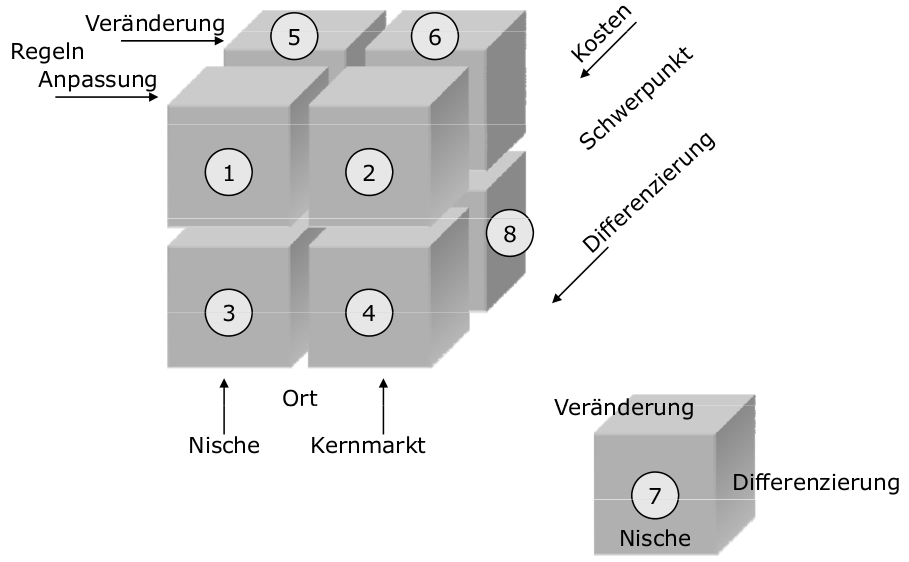
\includegraphics[scale=0.3]{bilder/strategische_optionen.png}
 \end{center}
\end{figure}
%%%%%%%%%%%%%%%%%%%%%%%%%%%%%%%%%%%%%%%

Überlegungen nur sinnvoll wenn Unternehmen in mehreren Geschäftsfeldern tätig ist oder eine Erweiterung auf mehrere geschäftsfelder geplant wird. 
Die möglichen Optionen sind:

\subsubsection*{Diversifikation} 
%%%%%%%%%%%%%%%%%%%%%%%%%%%%%%%%%%%%%%%
%% Bild: Diversifikation
\begin{figure}[h]
 \begin{center}
   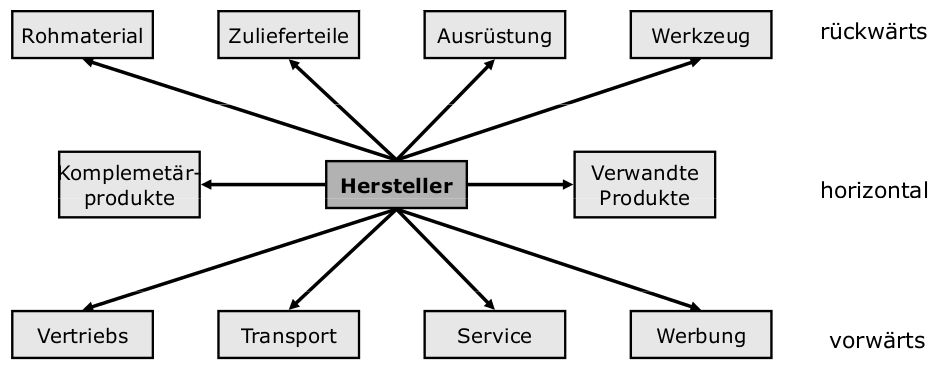
\includegraphics[scale=0.3]{bilder/diversifikation.png}
 \end{center}
\end{figure}
%%%%%%%%%%%%%%%%%%%%%%%%%%%%%%%%%%%%%%%
\newpage

\subsubsection*{Portfolio-Strategien} 

\textbf{?}: hohes Wachstum, aber relativ viel Konkurrenz\\
\textbf{$\star$}: großer Anteil und schnell wachsender Markt (bspw. Tablet-Produkte)\\
\textbf{Desinvestition}: schlecht, kein Wachstum und keine Anteile am Markt (Porter: "`nicht wachsender Markt"')\\ 
\textbf{Abschöpfung}: hoher Anteil, Wachstum stagniert ("`Milchkuh melken"')

%%%%%%%%%%%%%%%%%%%%%%%%%%%%%%%%%%%%%%%
%% Bild: Portfolio
\begin{figure}[h]
 \begin{center}
   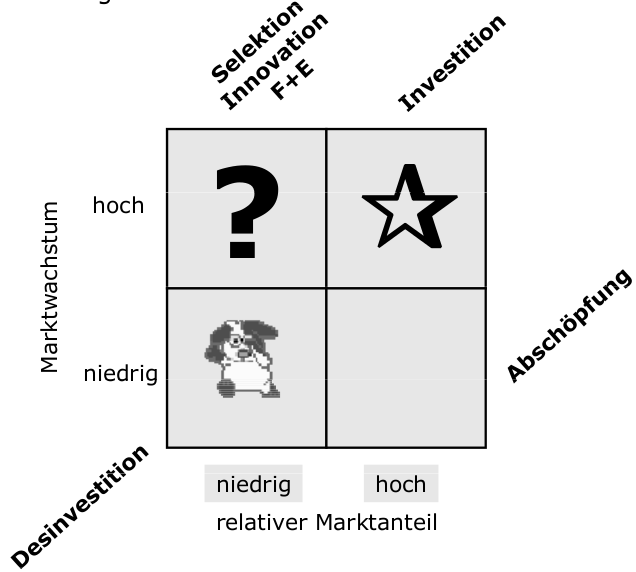
\includegraphics[scale=0.3]{bilder/portfolio.png}
 \end{center}
\end{figure}
%%%%%%%%%%%%%%%%%%%%%%%%%%%%%%%%%%%%%%%
\begin{center}
Alle 3 Diagramme müssen zueinander ins Verhältnis gebracht werden! $\downarrow$
\end{center}
%%%%%%%%%%%%%%%%%%%%%%%%%%%%%%%%%%%%%%%
%% Bild: Portfolio
\begin{figure}[h]
 \begin{center}
   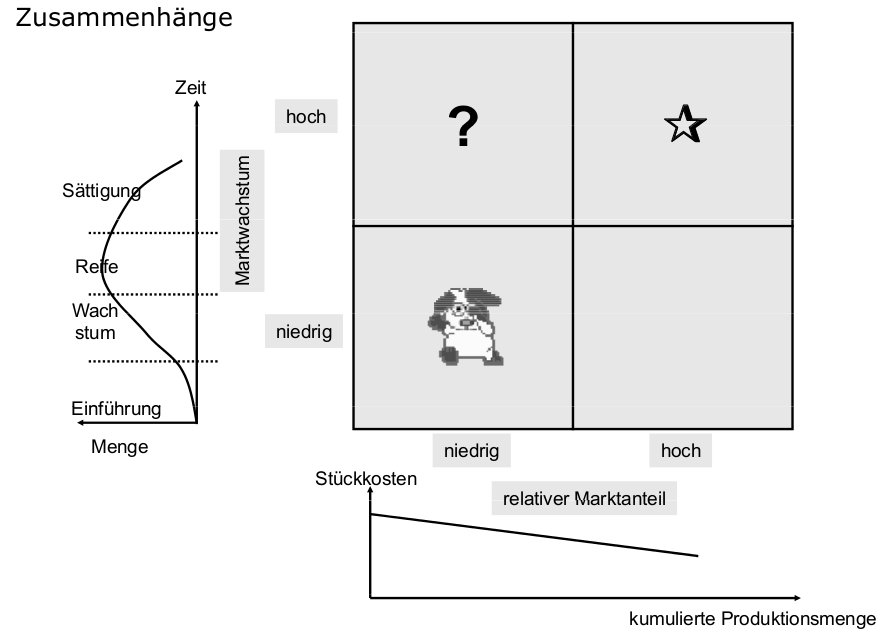
\includegraphics[scale=0.3]{bilder/portfolio_ext.png}
 \end{center}
\end{figure}
%%%%%%%%%%%%%%%%%%%%%%%%%%%%%%%%%%%%%%%

\subsubsection*{Internationalisierung} 
Ausdehnung der Geschäftstätigkeiten über Ländergrenzen hinweg, i.d.R. gleiche Produkt

National agierendes Unternehmen\\ 
\textit{Wie soll Markteintritt erfolgen?}
\begin{itemize}
	\item Export
	\item Lizenzvergabe oder Franchising
	\item Direktinvestition oder Akquisition
\end{itemize}

%% Randnotiz	
\mpar{\textcolor{red}{Steuern/Gesetzte nehmen Einfluss}}
International agierendes Unternehmen\\
\textit{Unterscheidung}\\
\begin{itemize}
	\item Globalisierung: das selbe Produkt und die selbe Wettbewerbsstrategie (diverse Ausführungen)
	\item Regionalisierung: Differenzierung des Produkts/Strategie
\end{itemize}

\subsubsection*{Kernkompetenzorientierung} 
Übergreifendes Qualifikationspotential, welches in verschiedenen Geschäftsfeldern den Aufbau von Wettbewerbsvorteilen ermöglicht

Merkmale von Kernkompetenzen:
\begin{itemize}
	\item Unternehmensweiter Geltungsbereich
	\item Dauerhafte Quelle von Wettbewerbsvorteilen
	\item historische Entwicklung
	\item kollektives Wissen
	\item Ressourcenwettbewerb
\end{itemize}
$\rightarrow$ Potentiale ausnutzen

\subsection{Strategische Wahl}
Auswahl der für das Unternehmen optimalen Strategie. Hierzu werden Beurteilungsgrößen herangezogen:
\begin{itemize}
	\item ökonomische Ziele
	\item Machbarkeit
	\item Akzeptanz
	\item ethische Vertretbarkeit
\end{itemize}
Dabei können verschiedene Probleme auftreten. Erfolge einer Strategie sind immer unsicher und ökonomische Auswirkungen immer nur schätzbar. Der "`Wert"' einer Strategie teilweise nicht quantifizierbar. Auswahlprozess ist komplex und nur teilweise rational.
 
\subsubsection*{Einflussfaktoren}

%%%%%%%%%%%%%%%%%%%%%%%%%%%%%%%%%%%%%%%
%% Bild: Portfolio
\begin{figure}[h]
 \begin{center}
   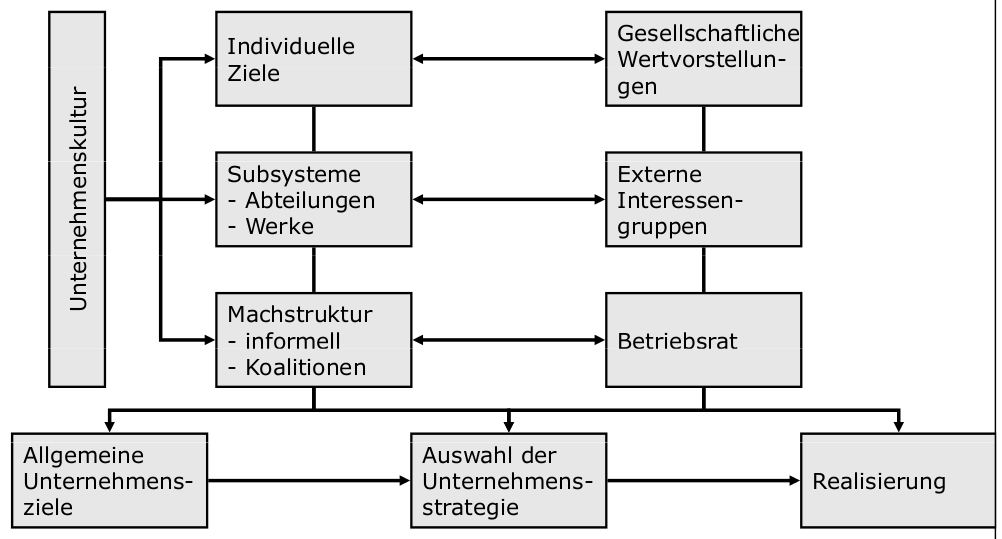
\includegraphics[scale=0.3]{bilder/strategische_einflussfaktoren.png}
 \end{center}
\end{figure}
%%%%%%%%%%%%%%%%%%%%%%%%%%%%%%%%%%%%%%%

\subsection{Strategieimplementation}
\underline{Drei} verschieden Punkte:

\subsubsection*{Strategische Maßnahmen}
\textit{"`structure follows strategy"'}\\
Kontingenztheorethischer Ausgangspunkt


\subsubsection*{Strategische Programme}
\textit{"`multidimensionale"' Zielsetzung}\\
Konkretisierung der Strategien in die einzelnen organisatorischen Bereiche und Ermittlung der kritischen Bereiche


\subsubsection*{Menschen/Führungssysteme}
\textit{"`strategy follows structure/personnel policy"'}\\
Strategische Personalplanung und -entwicklung sowie Problematik der Unternehmenskultur

$\rightarrow$ Balanced Scorecard

%%%%%%%%%%%%%%%%%%%%%%%%%%%%%%%%%%%%%%%
%% Bild: Portfolio
\begin{figure}[h]
 \begin{center}
   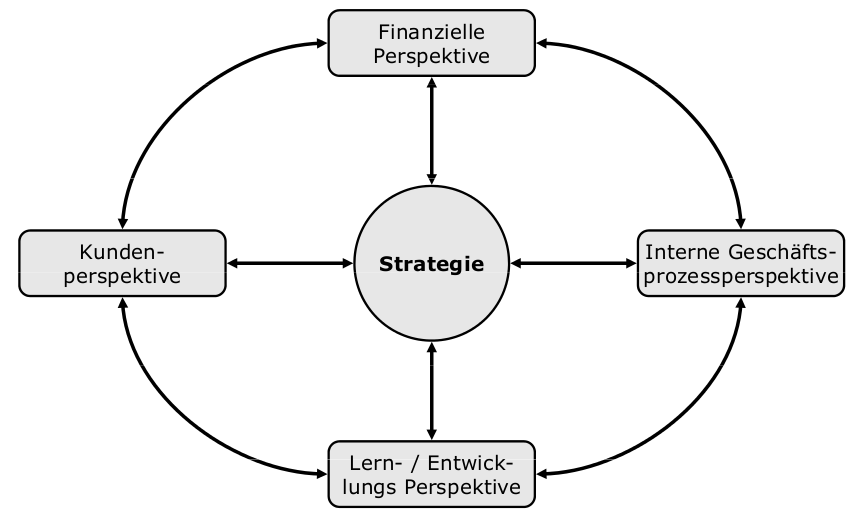
\includegraphics[scale=0.3]{bilder/strategische_balancedscorecard.png}
 \end{center}
\end{figure}
%%%%%%%%%%%%%%%%%%%%%%%%%%%%%%%%%%%%%%%

%%%%%%%%%%%%%%%%%%%%%%%%%%%%%%%%%%%%%%%
%% Bild: Portfolio
\begin{figure}[h]
 \begin{center}
   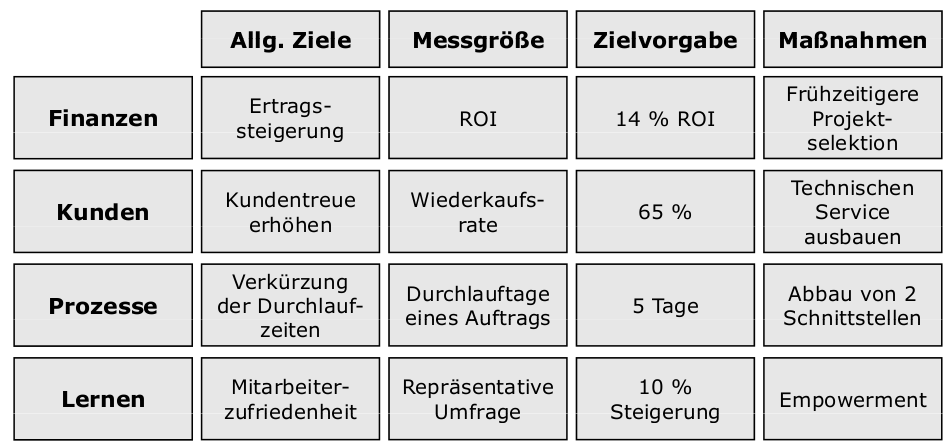
\includegraphics[scale=0.3]{bilder/strategische_balancedscorecard2.png}
 \end{center}
\end{figure}
%%%%%%%%%%%%%%%%%%%%%%%%%%%%%%%%%%%%%%%
\subsubsection*{Strategische Organisationsgestaltung}

\begin{tabular}{|l|l|}
\hline 
Einprodukt & Funktional/zentralisiert \\ 
\hline 
Verwandte Diversifikation & Divisional/dezentralisiert \\ 
\hline 
Konglomerate Diversifikation & Holding/stark dezentralisiert \\ 
\hline 
\end{tabular} 

Hat einen situativen Ansatz (Kontingent Ansatz). Bildung strategischer Geschäftseinheiten (SGE) in Anlehnung an die strategischen Geschäftsfelder. Mit Beachtung der Kernkompetenzen.

\subsubsection*{Strategische Personalpolitik}
Unterliegen Aspekten der Unternehmenskultur. Rückschlüsse der Personalentwicklung auf strategische Planung.

\subsection{Strategische Kontrolle}

%%%%%%%%%%%%%%%%%%%%%%%%%%%%%%%%%%%%%%%
%% Bild: Portfolio
\begin{figure}[h]
 \begin{center}
   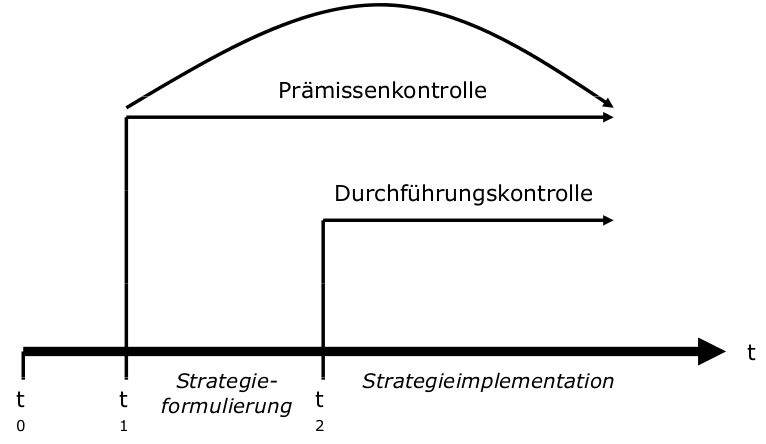
\includegraphics[scale=0.3]{bilder/strategische_kontrolle1.png}
 \end{center}
\end{figure}
%%%%%%%%%%%%%%%%%%%%%%%%%%%%%%%%%%%%%%%

%%%%%%%%%%%%%%%%%%%%%%%%%%%%%%%%%%%%%%%
%% Bild: Portfolio
\begin{figure}[h]
 \begin{center}
   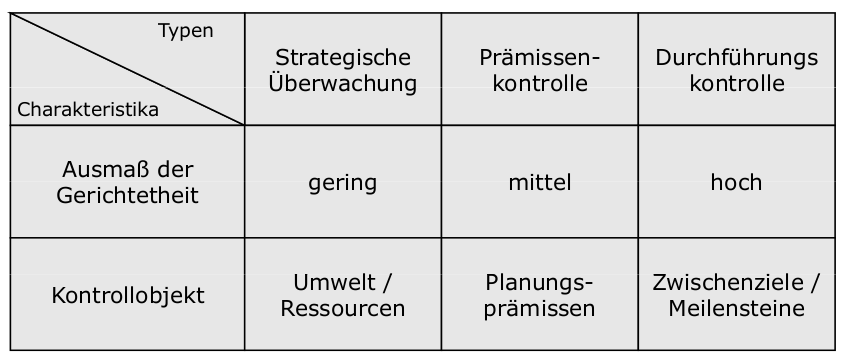
\includegraphics[scale=0.3]{bilder/strategische_kontrolle2.png}
 \end{center}
\end{figure}
%%%%%%%%%%%%%%%%%%%%%%%%%%%%%%%%%%%%%%%
\newpage

\subsection{Zusammenhänge der strategischen und operativen Planung}
%%%%%%%%%%%%%%%%%%%%%%%%%%%%%%%%%%%%%%%
%% Bild: Portfolio
\begin{figure}[h]
 \begin{center}
   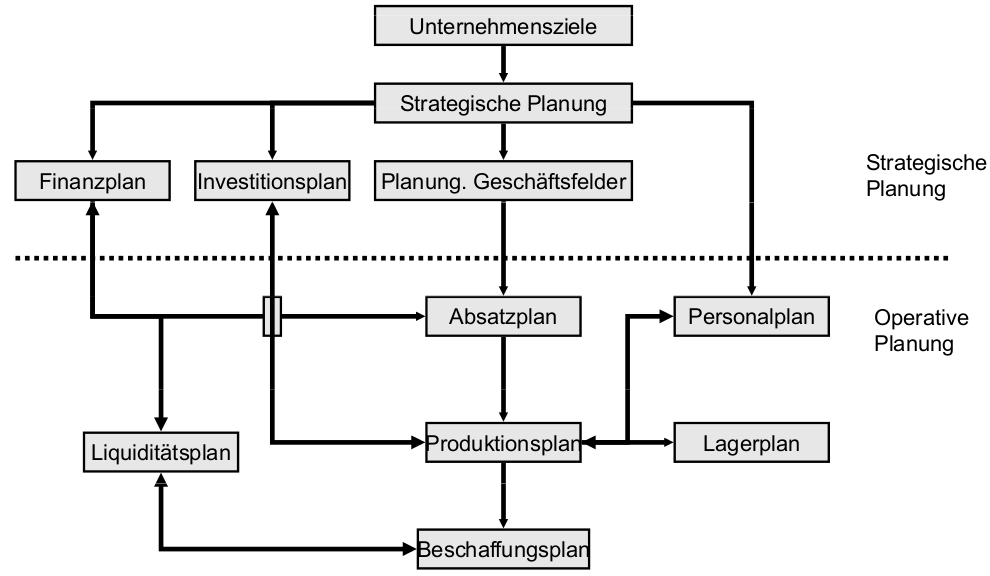
\includegraphics[scale=0.3]{bilder/zusammenhang_strop.png}
 \end{center}
\end{figure}
%%%%%%%%%%%%%%%%%%%%%%%%%%%%%%%%%%%%%%%



%%%%%%%%%%%%%%%%%%%%%%%%%%%%%%%%%%%%%%%%%%%%%%%%%%%%%%%%%%%%%%%%%%%%%%%%%%%%%%%%%%%%%%%%%%%%%%%%%%%%%%%%%%%%%%%%%%%%%%%%%%%%%%%%%%%%%%%%%%%%%%%%%%%%%%%%%%%%%%%%%%%%%%%%%%%%%%%%%%%%%%%%%%%%%%%%%%%%
\newpage
\section{Absatz}

\subsection{Grundlagen}
Dient der Leistungsverwertung: Suche nach Abnehmern, Physische Distribution der Ware

x-Rs der Absatzwirtschaft:
\begin{itemize}
	\item richtige Ware
	\item richtige Menge
	\item richtige Qualität
	\item richtige Zeit
	\item richtiger Ort
\end{itemize}
$\rightarrow$ steigender Stellenwert des Absatzes

Minimale Fehlmengenkosten + Minimale Bestandskosten $\rightarrow$ Formel
\begin{equation}
\text{Servicegrad} = \frac{\text{Anzahl der befriedigten Bedarfsanforderungen}}{\text{Anzahl aller Bedarfsanforderungen}} \cdot 100\%
\end{equation}
%%%%%%%%%%%%%%%%%%%%%%%%%%%%%%%%%%%%%%%
%% Bild: Portfolio
\begin{figure}[h]
 \begin{center}
   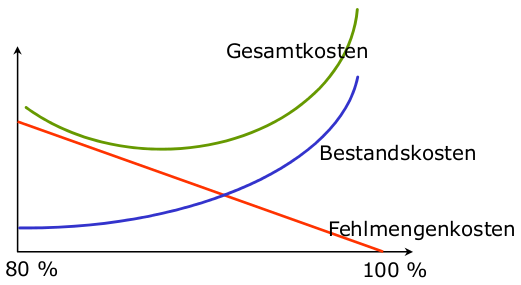
\includegraphics[scale=0.3]{bilder/servicegrad.png}
 \end{center}
\end{figure}
%%%%%%%%%%%%%%%%%%%%%%%%%%%%%%%%%%%%%%%

Erweiterung des Absatzbegriffs $\rightarrow$ Marketing\\ 
(= Konzeption der Unternehmensführung, die zur Erreichung der Unternehmensziele alle betrieblichen Aktivitäten konsequent auf die Erfordernisse des Absatzmarktes ausrichtet)

Aspekte des Marketings:
\begin{itemize}
	\item \textbf{Maxime}: Kunde als Ziel der Bemühungen
	\item  \textbf{Konzept}: geplanter und systematischer Einsatz der Instrumente zur Marktbeeinflussung und Gestaltung
	\item \textbf{Methode}: systematische Entscheidungsfindung und planmäßiges Vorgehen unter Einsatz wissenschaftlicher Methoden
\end{itemize}

\textbf{Entwicklung von Merketingstrategien/Wachstumsstrategien} 

%%%%%%%%%%%%%%%%%%%%%%%%%%%%%%%%%%%%%%%
%% Bild: Portfolio
\begin{figure}[h]
 \begin{center}
   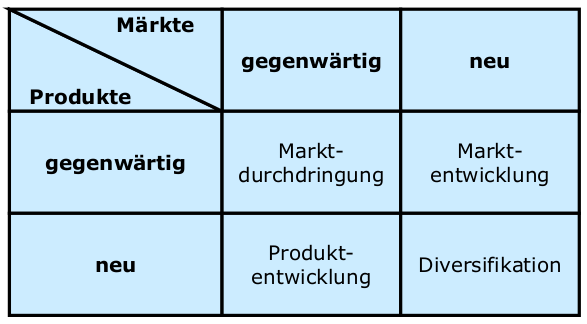
\includegraphics[scale=0.3]{bilder/marketingstrategien.png}
 \end{center}
\end{figure}
%%%%%%%%%%%%%%%%%%%%%%%%%%%%%%%%%%%%%%%

\textbf{Marktdurchdringung} (Abschöpfen des Marktpotentials)\\
...durch Erhöhung der Produktverwendung bei bestehenden Kunden\\
...durch Gewinnung von neuen Kunden\\
...durch Gewinnung von "`nicht"'-Verwendern\\

\textbf{Marktentwicklung} (Platzieren vorhandener Produkte in neuen Märkten)\\
Regionale Ausdehnung, neue Zielgruppen und Preisdifferenzierung

\textbf{Produktentwicklung} (Entwicklung neuer Produkte)\\
Innovationen und neue Produktvarianten

%% Randnotiz	
\mpar{\textcolor{red}{risikoreichste Wachstumstrategie}}

\textbf{Diversifikation} (Expansion in neue Geschäftsbereiche)\\
Horizontal: Erweiterung des Produktprogramms, mit ursprünglichem in sachlichem Zusammenhang\\
Vertikal: Vergrößerung der Tiefe des Produktprogramms (Vorwärtsintegration $\leftrightarrow$ Rückwärtsintegration)\\
Lateral: gänzlich neue Markt- und Produktgebiete (risikoreich)\\

\subsection{Marktforschung}
Beschaffung, Aufbereitung und Analyse von Informationen über Absatzmärkte zur Festlegung des optimalen Marketing-Mix

\textbf{Marketing-Mix}: (=optimale Abstimmung der Marketing-Instrumente zur Erreichnung der Ziele)\\
Produkt-. Preis-, Distributions- und Werbepolitik

\subsubsection*{Aufgaben}

\textbf{Analyse}
\begin{itemize}
	\item Erforschung der Grundstruktur des Marktes
	\item Zeitpunktbezogen 
\end{itemize}

\textbf{Beobachtung}
\begin{itemize}
	\item dynamische Komponente
	\item wesentliche Markteigenschaften (z.B. Konsolidierungen)
	\item A-Teile 
\end{itemize}

\textbf{Prognose}
\begin{itemize}
	\item Antizipation der zukünftigen Entwicklung wichtiger Trends (z.B. Substitutionsgüter)
	\item problematisch
\end{itemize}

\subsubsection*{Vorgehen}
\textbf{1. Zieldefinition}\\
Zweck der Untersuchung, Art, Ausmaß und Qualität der zu beschaffenden Information

\textbf{2. Wahl des Forschungsdesigns} - Grundsätzlicher Aufbau der Studie:
\begin{itemize}
	\item Explorativ (Gewinnung qualitativer Daten als Basisinformation)
%% Randnotiz	
\mpar{\textcolor{red}{Beispiel: "`Welche Eigenschaften muß eine Kaffeesorte für ältere Menschen aufweisen?"'}}
	\item Deskriptiv (Quantitative Beschreibung von Marktgegebenheiten, z.B. Absatzzahlen und Entwicklung des Marktanteils)
	\item Kausalanalytisch (Zusammenhänge zwischen Marktgegebenheiten, z.B. Wirkung der Verpackungsgestaltung auf den Marktanteil)
\end{itemize}

\textbf{3. Informationsgewinnung} - Wahl der Methode und des Umfangs der Untersuchung:\\
Primärforschung und Sekundärforschung

\textbf{4. Auswertung der Information} - Zielbezogene Analyse der erhobenen Daten:\\
Univariante Verfahren: Ermittlung einer Variablen (z.B. Kundenprofil eines Supermarkts)\\
Multivariante Verfahren: Ermittlung der Zusammenhänge mehrerer Variablen (z.B. Ladenöffnungszeiten und Eigenschaften der Käufergruppe)

\textbf{5. Ableiten von Konsequenzen auf den Marketing-Mix}

\subsubsection*{Methoden}

%%%%%%%%%%%%%%%%%%%%%%%%%%%%%%%%%%%%%%%
%% Bild: Portfolio
\begin{figure}[h]
 \begin{center}
   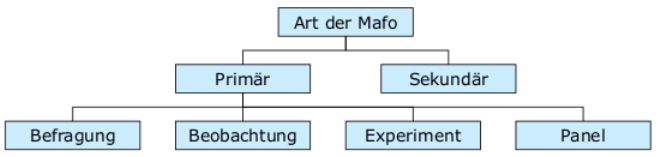
\includegraphics[scale=0.3]{bilder/methoden.png}
 \end{center}
\end{figure}
%%%%%%%%%%%%%%%%%%%%%%%%%%%%%%%%%%%%%%%
\textbf{Befragung} - Festzulegen sind:
\begin{itemize}
	\item Zielgruppe
	\item Befragungsgegenstand
	\item Art der Befragung
	\item Standardisierung
	\item Häufigkeit
\end{itemize}

\textbf{Beobachtung} - "`Zielgerichtete und planmäßige Erfassung von sinnlich wahrnehmbaren Sachverhalten im Augenblick ihres Auftretens"'\\
Festzulegen sind:
\begin{itemize}
	\item Bewusstseinsgrad des Beobachteten
	\item Partizipationsgrad des Beobachteten
	\item Standardisierungsgrad
	\item Wahrnehmungs- und Registrierungsform
\end{itemize}

\textbf{Experiment} - Studie von Sachverhalten unter vorher exakt festgelegten Rahmenbedingungen\\
$\rightarrow$ Isolierte Variation eines bestimmten Faktors

\textbf{Panel} - wiederholte Befragung eins feststehenden Personenkreises
$\rightarrow$ Ermittlung der Veränderungen des Zielgruppenverhaltens im Zeitablauf

\subsection{Instrumente}

%%%%%%%%%%%%%%%%%%%%%%%%%%%%%%%%%%%%%%%
%% Bild: Portfolio
\begin{figure}[h]
 \begin{center}
   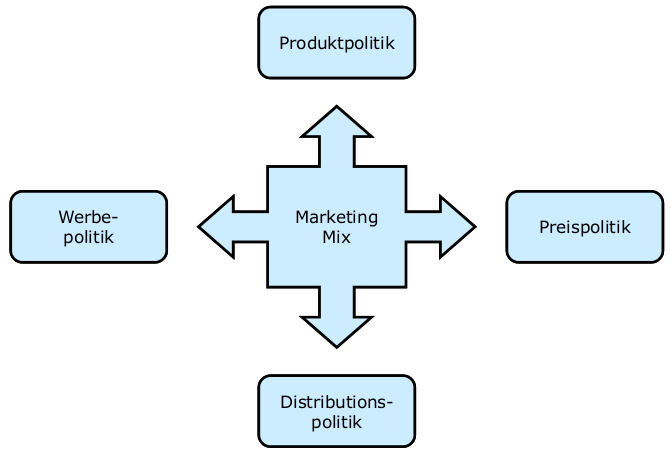
\includegraphics[scale=0.3]{bilder/instrumente_produktpolitik.png}
 \end{center}
\end{figure}
%%%%%%%%%%%%%%%%%%%%%%%%%%%%%%%%%%%%%%%

\subsubsection{Produktpolitik}
Umfasst alle Überlegungen und Entscheidungen marktlicher Natur, die sich auf die Gestaltung von Art und Beschaffenheit der angebotenen Güter beziehen

\textbf{Leitfragen}\\
\textit{Welche Art von Erzeugnissen wünscht der Markt jetzt und in Zukunft?}\\
\textit{Welche Beschaffenheit müssen die Güter in den Augen der Nachfrager aufweisen?}

\textbf{Produktgestaltung}\\
Produktneuheit, Betriebsinnovation (Konkurrenzprodukt existiert bereits), Produktvariation

\textbf{Bedeutung}\\
\begin{itemize}
	\item hohe Bedeutung, da bedeutsam für den zukünftigen Unternehmenserfolg
	\item Risiko bei Nachahmung durch die Konkurrenz
\end{itemize}
$\rightarrow$ ca. 75\% aller Umsätze mit Produkt\\
$\rightarrow$ ca. 80\% der Neueinführungen enden als Flop

\textbf{Gestaltungsbereiche}\\
"`Innere Werte"'(Material, Verarbeitungs- und Funktionsqualität) und Äußeres (Design des Produktes/Verpackung)

\textbf{Wertanalyse}\\
Betrachtet Produkt als Bündel von Funktionen, gesucht ist die beste Kombination der Eigenschaften aus Sicht des Verbrauchers\\
Zentrale Fragen:\\
\textit{Wie viel kostet eine bestimmte Funktion des Produktes?}\\
\textit{Wo lassen sich Kosten einsparen?}
\textit{Welche Eigenschaft/Funktion lässt sich mit geringem Aufwand ändern?}
%%%%%%%%%%%%%%%%%%%%%%%%%%%%%%%%%%%%%%%
%% Bild: Portfolio
\begin{figure}[h]
 \begin{center}
   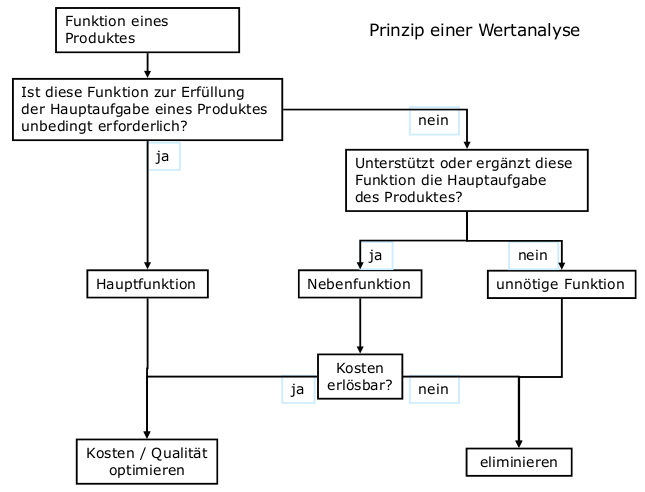
\includegraphics[scale=0.3]{bilder/wertanalyse.png}
 \end{center}
\end{figure}
%%%%%%%%%%%%%%%%%%%%%%%%%%%%%%%%%%%%%%%

\textbf{Kritik}
\begin{itemize}
	\item Produktinnovationen per se schaffen keinen dauerhaften Wettbewerbsvorteil (Innovationsfalle)
	\item Geplante physische Veralterung
	\item Variationen im Produkt oder seinem Design ziehen Änderungen in der Produktion nach sich
	\item "`Etikettenschwindel"'
\end{itemize}

\subsubsection{Preispolitik}
Alle Entscheidungen, die sich auf das Entgelt für die Angebotsleistung beziehen und damit zusammenhängend auf die Konditionen, unter denen das Entgelt zu entrichten ist

\textbf{Umfang}
\begin{itemize}
	\item Fixierung des Listenpreises
	\item Zahlungs- und Lieferungsbedingungen
	\item die mit dem Kauf zusammenhängenden Serviceleistungen
	\item Leistungen im After Sales Bereich
\end{itemize}

\textbf{Bedeutung}
\begin{itemize}
	\item Zunehmende Deregulierung
	\item Internationalisierung
	\item Produktdifferenzierung
\end{itemize}

\textbf{Kostenorientierte Preispolitik im Handel}
%%%%%%%%%%%%%%%%%%%%%%%%%%%%%%%%%%%%%%%
%% Bild: Portfolio
\begin{figure}[h]
 \begin{center}
   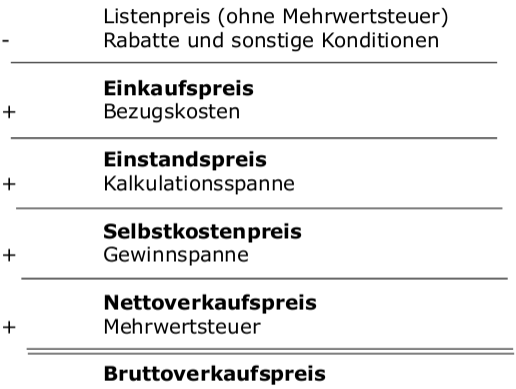
\includegraphics[scale=0.3]{bilder/kostenorientierte_preispolitik.png}
 \end{center}
\end{figure}
%%%%%%%%%%%%%%%%%%%%%%%%%%%%%%%%%%%%%%%
\newpage 

\textbf{Kostenorientierte Preispolitik beim Hersteller}
%%%%%%%%%%%%%%%%%%%%%%%%%%%%%%%%%%%%%%%
%% Bild: Portfolio
\begin{figure}[h]
 \begin{center}
   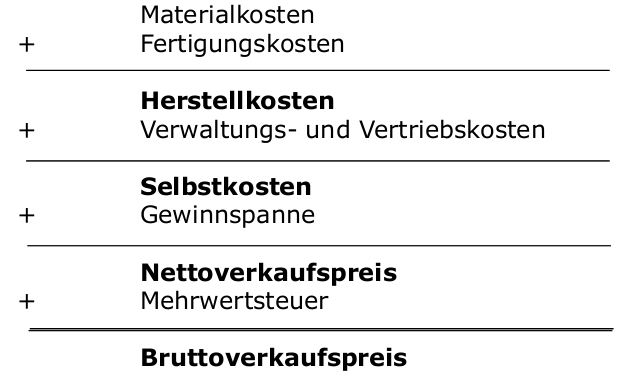
\includegraphics[scale=0.3]{bilder/kostenorientierte_preispolitik2.png}
 \end{center}
\end{figure}
%%%%%%%%%%%%%%%%%%%%%%%%%%%%%%%%%%%%%%%

\textbf{Möglichkeiten der Preisbeeinflussung}
\begin{itemize}
	\item Preisdifferenzierung (Abnehmer-/Anbieterstufe, Niveau der Einkaufsstätte)
	\item Zu- und Abschläge (Mindermengenzuschlag)
	\item Rabatte (Natural-/Funktionsrabatt, Mengenrabatt und Staffelpreise)
	\item Bonus
\end{itemize}

\textbf{Preisgestaltung - Zahlungsbedingungen/Finanzierungsangebote}\\
Die Zahlungsbedingungen legen den Zeitpunkt fest, an dem der Kunde die Zahlung zu erbringen hat.
%%%%%%%%%%%%%%%%%%%%%%%%%%%%%%%%%%%%%%%
%% Bild: Portfolio
\begin{figure}[h]
 \begin{center}
   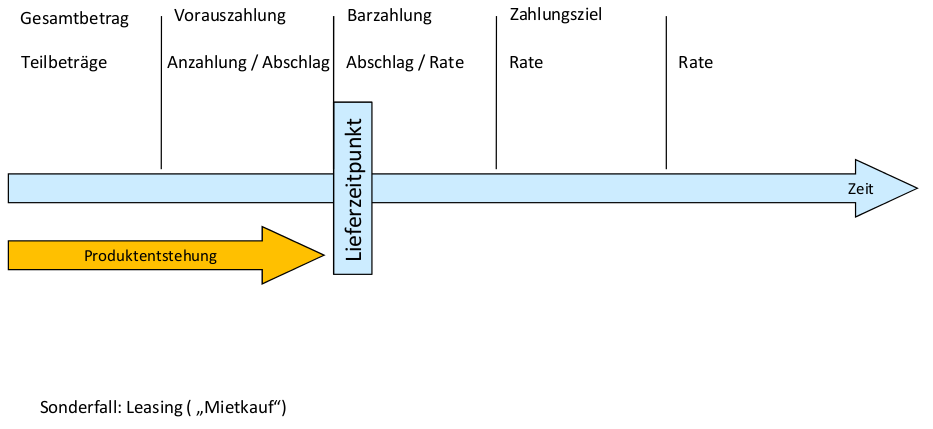
\includegraphics[scale=0.3]{bilder/preisgestaltung.png}
 \end{center}
\end{figure}
%%%%%%%%%%%%%%%%%%%%%%%%%%%%%%%%%%%%%%%

\textbf{Ziele/Anlässe}
\begin{itemize}
	\item Veränderungen der Absatzmengen oder -zeiten
	\item Selektion von Abnehmergruppen
	\item Veränderungen in der Bedarfs- oder Qualitätsstruktur der Nachfrager 
\end{itemize}

\textbf{Strategien}\\
Hochpreis, Niedrigpreis und Abschöpfungsstrategien

\textbf{Kritik}
\begin{itemize}
	\item im Polypol stellt Preis ein Datum dar $\rightarrow$ Indiz für Vollkommenheit des Marktes
	\item (sehr) kurzfristiges Instrument
	\item Preis ist markt- und unternehmensabhängig 
	\item Preisänderung ist vorwiegend psychologisches Signal
	\item kurzfristige Preissenkung haben Auswirkungen auf die gesamte Logistikkette
\end{itemize}

\subsubsection{Distributionspolitik}
Ist die grundsätzliche Gestaltung des verwenderbezogenen Vertriebskonzepts bei dezentralisierter Marktbearbeitung

\textbf{Einflussfaktoren}
\begin{itemize}
	\item Produktbezogen
	\item Verwenderbezogen
	\item Konkurrenzbezogen
\end{itemize}

\textbf{Gestaltungsmöglichkeiten}

Direktvertrieb
\begin{itemize}
	\item Verkaufsniederlassung (wirtschaftlich und rechtlich unselbständige Unternehmen)
	\item Vertriebsgesellschaften (rechtlich selbständige Gesellschaften)
	\item Reisende (Angestellte des Unternehmens)
	\item Online-Shop
\end{itemize}

Absatzhelfer\\
rechtlich und wirtschaftlich selbständige Unternehmen, die Kontaktanbahnung und Auftragsakquisition übernehmen
\begin{itemize}
	\item Handelsvertreter (Gewerbetreibende, der in fremden Name und auf fremde Rechnung tätig ist)
	\item Kommissionär (Selbständiger gewerbetreibender, ist unter eigenem Namen für fremde Rechnung tätig)
	\item (Handels) Makler (vermittelt gewerbsmäßig Vertragsabschlüsse für Dritte)
\end{itemize}

Absatzmittler
Handelsbetriebe die in eigenem Namen und auf eigene Rechnung Waren beschaffen und veräußern
\begin{itemize}
	\item Großhandel (Kauf und Verkauf an weitere Händler, Großabnehmer und Weiterverarbeiter, unter Kaufleuten und große Mengen)
	\item Einzelhandel (Verkauf an Endverbraucher, Sortimentsbildung auf Basis haushaltsüblicher Mengen)
\end{itemize}

\textbf{Betriebsformen im Einzelhandel}
%%%%%%%%%%%%%%%%%%%%%%%%%%%%%%%%%%%%%%%
%% Bild: Portfolio
\begin{figure}[h]
 \begin{center}
   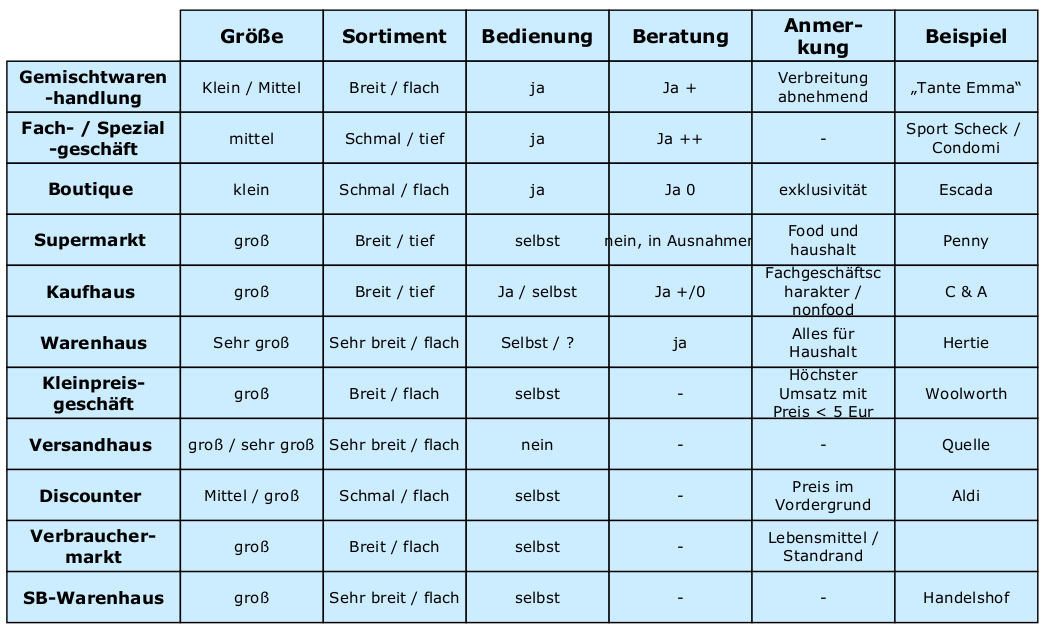
\includegraphics[scale=0.3]{bilder/betriebsformen_einzelhandel.png}
 \end{center}
\end{figure}
%%%%%%%%%%%%%%%%%%%%%%%%%%%%%%%%%%%%%%%

\newpage
\textbf{Struktur der Absatzwege}
%%%%%%%%%%%%%%%%%%%%%%%%%%%%%%%%%%%%%%%
%% Bild: Portfolio
\begin{figure}[h]
 \begin{center}
   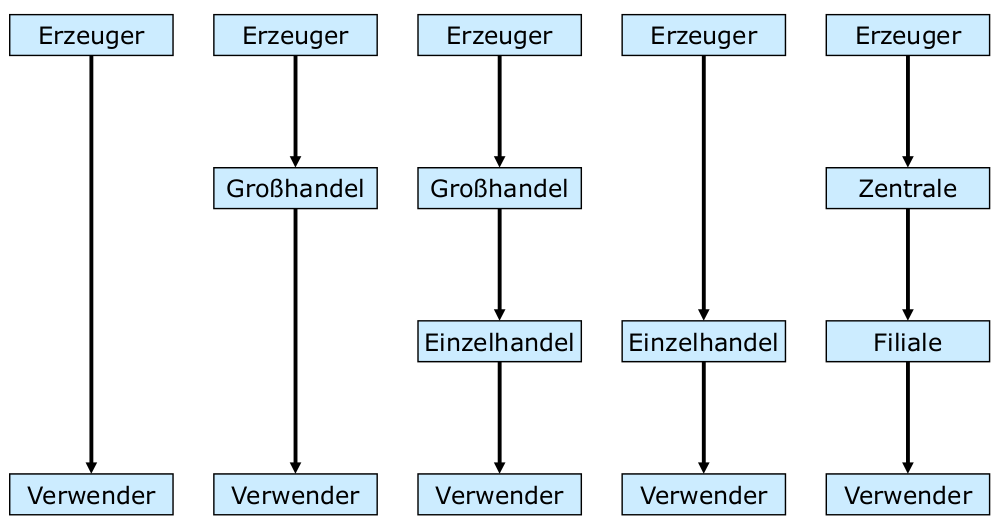
\includegraphics[scale=0.3]{bilder/absatzwege.png}
 \end{center}
\end{figure}
%%%%%%%%%%%%%%%%%%%%%%%%%%%%%%%%%%%%%%%

\textbf{Sortimentsfunktion des Handels}
%%%%%%%%%%%%%%%%%%%%%%%%%%%%%%%%%%%%%%%
%% Bild: Portfolio
\begin{figure}[h]
 \begin{center}
   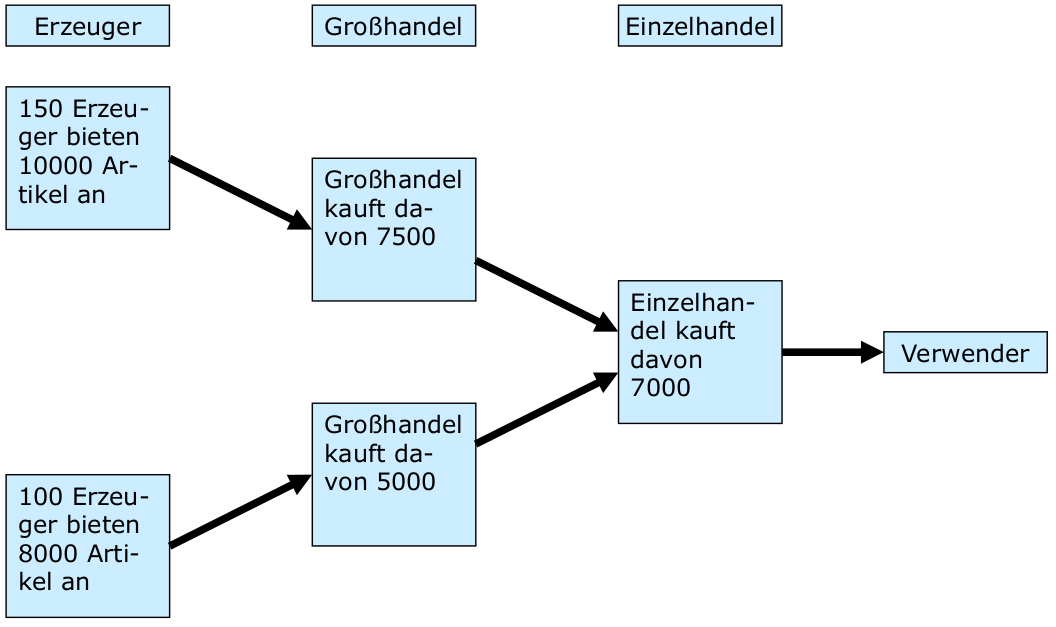
\includegraphics[scale=0.3]{bilder/sortimentsfunktion.png}
 \end{center}
\end{figure}
%%%%%%%%%%%%%%%%%%%%%%%%%%%%%%%%%%%%%%%
\newpage

\textbf{Vertragliche Abnehmerbedingungen}
\begin{itemize}
	\item Bindung der Einkaufs- und Lagerhaltungspolitik (Abnehmer verpflichtet sich bestimmte Menge/Sortiment abzunehmen oder vorrätig zu halten) 
	\item Vertriebsbindung (Bindung des Weiterverkäufers an bestimmte Zielgruppe/Vertriebsgebiet) 
	\item Preisbindung (mit Ausnahmen seit 1973 verboten, bspw. Bücher, Arzneimittel)
	\item Vertragshändlersystem (Händler benutzt Namen/Markenzeichen des Herstellers)
	\item Franchising (Bezahlung für Benutzung von Markenzeichen/Namen/Ausstattung, Gebietsschutz)
\end{itemize}

\textbf{Zusammenfassende Wertung}\\
Wahl der Distributionswege ist strategische Entscheidung, Handel fungiert als "`Gatekeeper"'. Ein bestehendes Distributionsnetz kann einen erheblichen Wettbewerbsfaktor darstellen, allerdings entstehen auch latente Bedrohungen durch neue Distributionswege.

\subsubsection{Werbepolitik}
Festlegung der Kommunikationsleistung des Unternehmens zur Steigerung des Absatzes der eigenen Produkte

\textit{$\>>$ Werbung ist die bewusste, meist unpersönliche, unaufgeforderte und einseitige Beinflussung überwiegend anonymer Personenkreise im Sinne des Werbetreibenden mittels Medien} 

\textbf{Werbemittel:} gestaltete und technisch fixierte Werbebotschaften\\
\textbf{Werbeträger:} Transportmedium des Werbemittels\\

\textbf{Werbepolitische Entscheidungen}
\begin{itemize}
	\item Festlegung der zu bewerbenden Ziel-/Produktgruppe  
	\item Fixierung der Werbethematik (Profil des Produkts, Positionierung gegenüber Konkurrenzprodukten)
	\item Ausmaß der Werbekontakte (Häufigkeit und Intervalle, Zeiten und Orte, Medien und Werbeträger)
	\item Ziele der Werbung (z.B. Steigerung des Bekanntheitsgrads)
\end{itemize}

\textbf{Betriebswirtschaftliche Aspekte}\\
Grundlegendes Problem: Messung des Werbeerfolgs - Aufwand $\leftrightarrow$ Ertrag\\
$\rightarrow$ Grenzkosten der Werbung = Grenzertrag der Werbung!!

Einflussfaktoren
\begin{itemize}
	\item Konkurrenz und Konjunktureinflüsse
	\item "`Erfolgsspaltung"' - \textit{Welcher Teil des Verkaufserfolgs ist auf die Werbung zurückzuführen?}
	\item "`Carry-Over-Effekt"' - \textit{Werbewirkung kann über den Zeitraum der Werbung hinaus anhalten}
	\item "`Spill-Over-Effekt"' - \textit{Erhöhung des Erfolgs von Konkurrenzprodukten}
	\item "`Verbundeffekte"' - \textit{Erhöhter Werbeaufwand und Kostendegressionseffekte in der Produktion}
\end{itemize}

\textbf{Durchführung der Werbung}\\
Ablauf
\begin{itemize}
	\item Erarbeitung der Werbekonzeption
	\item Gestaltung der Werbemittel
	\item Auswahl der Medien
	\item Streuung der Werbemittel
\end{itemize}

Zentrale Fragen\\
\textit{Welche Werbemittel sind von ihren Gestaltungsmöglichkeiten her für die Werbeaussage geeignet?}\\
\textit{Welche Werbeträger kommen grundsätzlich in Frage?} (Stil, Zielgruppe, Kosten, Zeitpunkt und Volumen)\\
\textit{Wie und in welchem Umfang muss gestreut werden?}\\

\textbf{Zusammenfassende Wertung}
\begin{itemize}
	\item Werbung ist vorwiegend ein psychologisches Problem (Spezialisten, weiche Faktoren)
	\item Werbung ist unvermeidlich "`Endlosschraube"'
	\item Werbung ist mit zunehmend steigendem finanziellen Aufwand verbunden
	\item Erfolgsmessung ist problematisch	
\end{itemize}

%%%%%%%%%%%%%%%%%%%%%%%%%%%%%%%%%%%%%%%%%%%%%%%%%%%%%%%%%%%%%%%%%%%%%%%%%%%%%%%%%%%%%%%%%%%%%%%%%%%%%%%%%%%%%%%%%%%%%%%%%%%%%%%%%%%%%%%%%%%%%%%%%%%%%%%%%%%%%%%%%%%%%%%%%%%%%%%%%%%%%%%%%%%%%%%%%%%%
\newpage
\section{Kosten- und Erfolgscontrolling}

\subsection{Grundlagen und Grundbegriffe}

\subsubsection*{Aufgaben}
\textbf{Rechnungswesen}\\
Unterscheidung zwischen:
\begin{itemize}
	\item Externes Rechnungswesen: Finanz-, Geschäftsbuchhaltung, Jahresabschluss
	\item Internes Rechnungswesen Kosten- und Leistungsrechnung (interne Entscheidungsprozesse)
\end{itemize}

\textbf{Aufgaben der Kosten- und Leistungsrechnung}\\
Erfassung anfallender Kosten und verursachungsgerechte Zurechnung der Kosten zu den Kostenträgern
\begin{itemize}
	\item Kalkulation der Herstell- und Selbstkosten
	\item Festsetzung der kurz- und langfristigen Preisuntergrenze
\end{itemize}
Wirtschaftlichkeitskontrolle
\begin{itemize}
	\item Vergleich von Plan-/Istkosten
\end{itemize}
Bereitstellung von Informationen für Entscheidungsrechnungen
\begin{itemize}
	\item z.B. Eigenfertigung und Fremdbezug, kostenoptimales Produktionsprogramm, usw.
\end{itemize}

\subsubsection*{Teilgebiete der Kostenrechnung}
%%%%%%%%%%%%%%%%%%%%%%%%%%%%%%%%%%%%%%%
%% Bild: Portfolio
\begin{figure}[h]
 \begin{center}
   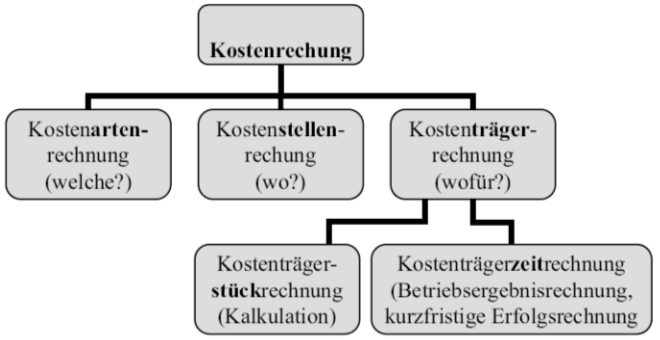
\includegraphics[scale=0.3]{bilder/kostenrechnung.png}
 \end{center}
\end{figure}
%%%%%%%%%%%%%%%%%%%%%%%%%%%%%%%%%%%%%%%

\subsubsection*{Aufwand und Kosten}
\textbf{Aufwand (Finanzbuchhaltung):} zu Anschaffungsausgaben bewerteter Güterverbrauch\\
\textbf{Kosten (Kostenrechnung):} bewerteter leistungsbezogener Güterverbrauch\\
\textbf{Gemeinsamkeiten:} Güterverbrauch, kein Gütertausch (Geld gegen Ware)\\
\textbf{Unterschiede:} Leistungsbezug der Kosten, Bewertung des Güterverbrauchs (Anschaffungswert gegen Wiederbeschaffungswert)

%%%%%%%%%%%%%%%%%%%%%%%%%%%%%%%%%%%%%%%
%% Bild: Portfolio
\begin{figure}[h]
 \begin{center}
   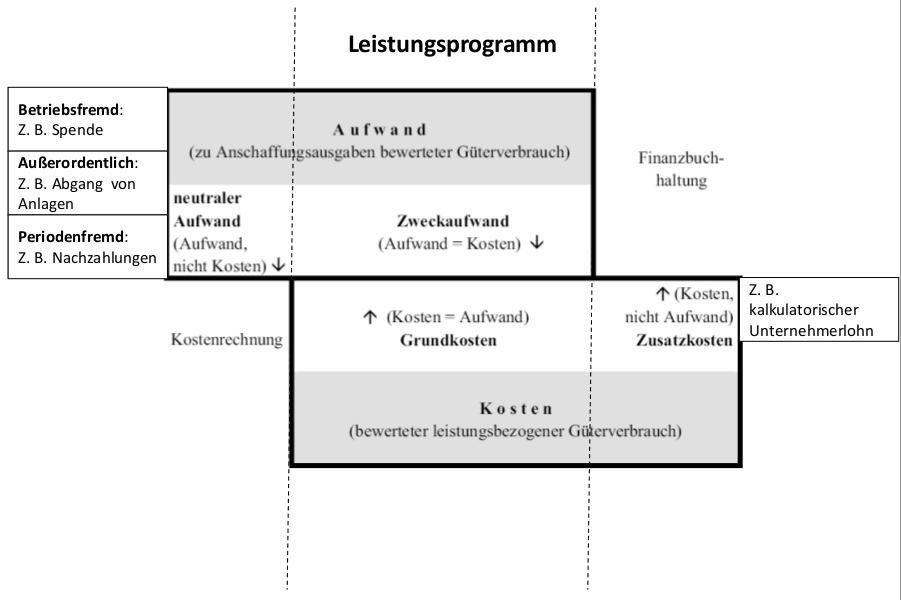
\includegraphics[scale=0.3]{bilder/leistungsprogramm.png}
 \end{center}
\end{figure}
%%%%%%%%%%%%%%%%%%%%%%%%%%%%%%%%%%%%%%%

\subsubsection*{Ertrag und Leistung}

\textbf{Ertrag (Finanzbuchhaltung)}\\
Bewertete Güterentstehung aller Art
\begin{itemize}
	\item Abgesetzte Erzeugnisse: Erlöse
	\item Gelagerte Erzeugnisse: Herstelleraufwand (=Herstellkosten)
\end{itemize}

\textbf{Leistung (Kostenrechnung)}\\
Bewertete betriebstypische Leistung
\begin{itemize}
	\item Innerbetriebliche Leistung (wird im Betrieb verbucht)
	\item Marktleistung (wird verkauft $\rightarrow$ Bewertung zu Verkaufspreisen)
\end{itemize}

\textbf{Neutraler Ertrag}\\
Ertrag der nicht betriebstypisch ist, wie z.B. Vermietung oder Wertpapiergeschäfte

\textbf{Zusatzleistung}\\
Erschaffung eines selbst genutzten Patents

%%%%%%%%%%%%%%%%%%%%%%%%%%%%%%%%%%%%%%%
%% Bild: Portfolio
\begin{figure}[h]
 \begin{center}
   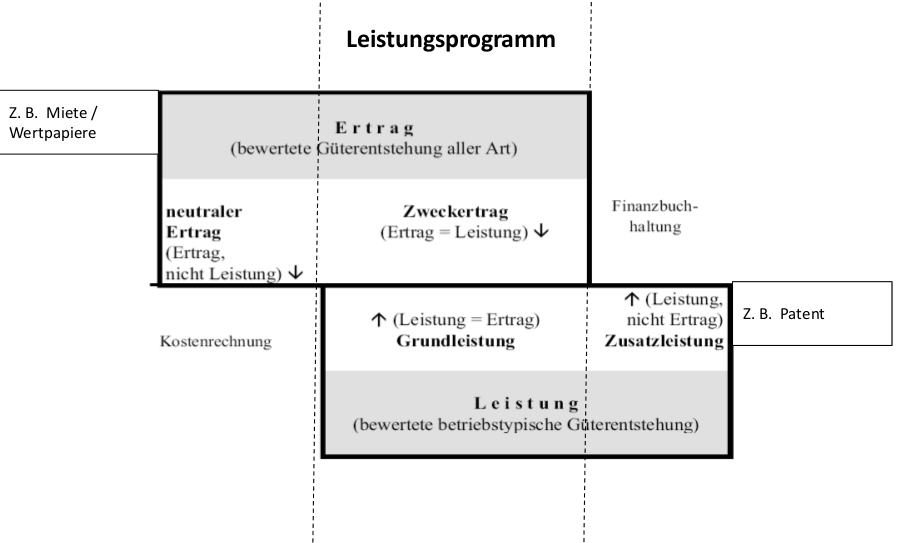
\includegraphics[scale=0.3]{bilder/leistungsprogramm2.png}
 \end{center}
\end{figure}
%%%%%%%%%%%%%%%%%%%%%%%%%%%%%%%%%%%%%%%

\subsection{Kostenartenrechnung}

\subsubsection*{Aufgaben und Gliederung der Kostenarten}

\textbf{Aufgaben}\\
Vollständige und überschneidungsfreie Erfassung der Kosten sowie Gliederung der Kostenarten bis zur Informationsweitergabe ans Kostenstellen- und Kostenträgerrechnung 

\textbf{Gliederung nach Art der verbrauchten Produktionsfaktoren (Primäre Kosten)}
\begin{itemize}
	\item Personalkosten (Löhn und Gehälter)
	\item Materialkosten (Roh- und Hilfsstoffe)
	\item Kalkulatorische Abschreibungen (Maschinen und Gebäude)
	\item Kalkulatorische Zinsen (Kapitalkosten)
	\item Fremdleistungskosten (Beratungskosten, Speditionskosten)
	\item Wagniskosten (Garantiekosten)
	\item Steuern (Grundsteuer)
\end{itemize}

%%%%%%%%%%%%%%%%%%%%%%%%%%%%%%%%%%%%%%%
%% Bild: Portfolio
\begin{figure}[h]
 \begin{center}
   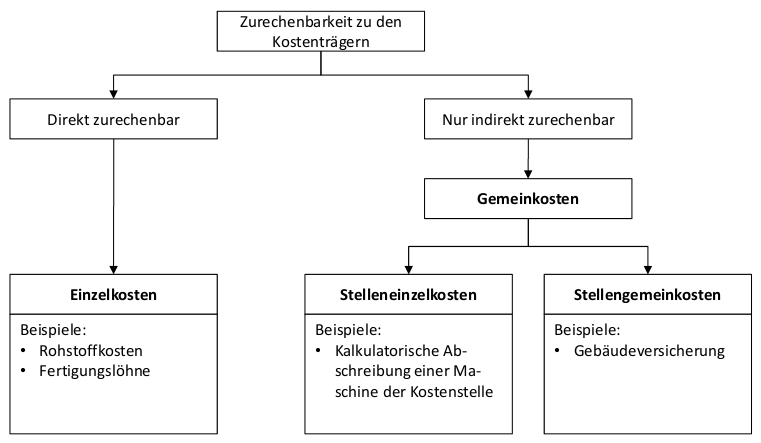
\includegraphics[scale=0.3]{bilder/primaerkosten.png}
 \end{center}
\end{figure}
%%%%%%%%%%%%%%%%%%%%%%%%%%%%%%%%%%%%%%%

\textbf{Unterscheidung der Kosten bei Beschäftigungsschwankungen}
%% Randnotiz
\mpar{\textcolor{red}{Fixkosten bleiben immer Fixkosten}}
\begin{itemize}
	\item Fixkosten (unabhängig von der Höhe der Beschäftigung, Aufrechterhaltung der Betriebs-/Leistungsbereitschaft)
	\item Sprungfixe Kosten (im Rahmen von Beschäftigungsintervallen immer konstant)
	\item Variable Kosten (abhängig von Beschäftigung)
\end{itemize}

\textbf{Zusammenhang Fixe/variable und Einzel-/Gemeinkosten}\\
Fixe Kosten sind immer Gemeinkosten und Einzelkosten sind immer Variabel
%%%%%%%%%%%%%%%%%%%%%%%%%%%%%%%%%%%%%%%
%% Bild: Portfolio
\begin{figure}[h]
 \begin{center}
   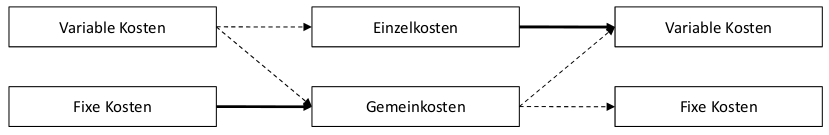
\includegraphics[scale=0.3]{bilder/zshkosten.png}
 \end{center}
\end{figure}
%%%%%%%%%%%%%%%%%%%%%%%%%%%%%%%%%%%%%%%
\newpage 

\subsubsection*{Personalkosten}
\textbf{Personalkosten und deren Verrechnung}
%%%%%%%%%%%%%%%%%%%%%%%%%%%%%%%%%%%%%%%
%% Bild: Portfolio
\begin{figure}[h]
 \begin{center}
   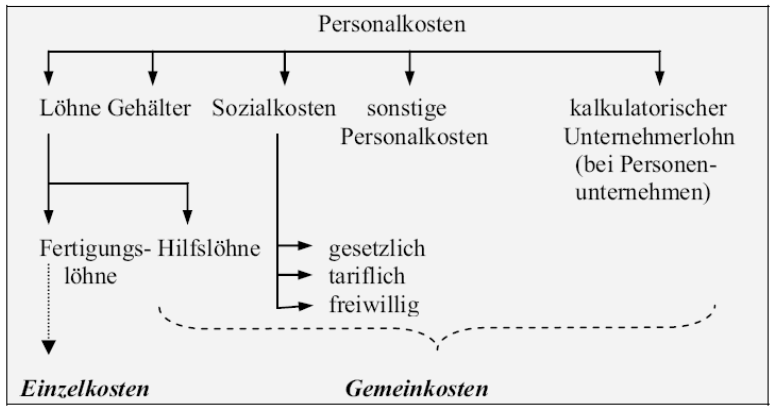
\includegraphics[scale=0.3]{bilder/personalkosten.png}
 \end{center}
\end{figure}
%%%%%%%%%%%%%%%%%%%%%%%%%%%%%%%%%%%%%%%

\subsubsection*{Materialkosten}
\textbf{Materialkosten und deren Verrechnung}
%%%%%%%%%%%%%%%%%%%%%%%%%%%%%%%%%%%%%%%
%% Bild: Portfolio
\begin{figure}[h]
 \begin{center}
   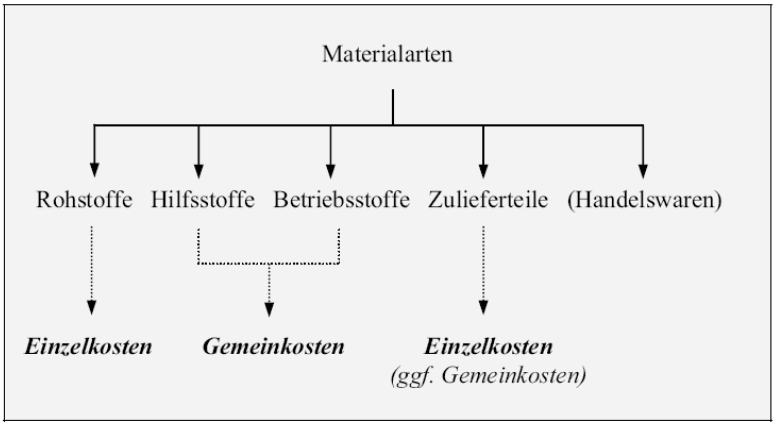
\includegraphics[scale=0.3]{bilder/materialkosten.png}
 \end{center}
\end{figure}
%%%%%%%%%%%%%%%%%%%%%%%%%%%%%%%%%%%%%%%

\textbf{Ermittlung des Materialverbrauchs}
Teilt sich in zwei veschiedene Arten:
%% Randnotiz	
	\mpar{\textcolor{red}{Kann ermittelt werden (bspw. durch Auftrag)}}
\begin{itemize}
	\item Ordentlicher Materialverbrauch = Summe der Menge auf Materialentnahmescheine
	\item Ausserordentlicher Verbrauch:\\
			\text{Ist-Anfangsbestand (laut Inventur)}\\
			\text{+ Ist-Zugang (laut Lieferscheine)}\\
			\text{- Ist-Verbrauch (laut Materialentnahmescheine)}\\
			\textbf{= Soll-Endbestand}\\
			\text{- Ist-Endbestand (laut Inventur)}\\
			\textbf{= ausserordentlicher Verbrauch}\\
\end{itemize}
%% Randnotiz	
	\mpar{\textcolor{red}{Inventur ist nötig}}
$\rightarrow$ die verbrauchten Mengen werden in der Regel mit durchschnittlichen Anschaffungspreisen bewertet ("`Verbrauchswerte"')

\subsubsection*{Kalkulatorische Kosten}
Unterscheidung zweier Arten: Kalkulatorische Abschreibungen/Zinsen


\textbf{Kalkulatorische Abschreibungen}
\begin{itemize}
	\item Betriebsmittel (Gebäude/Maschinen) sind langfristige nutzbare Produktionsfaktoren und müssen über mehrere Nutzungsjahre verteilt werden ("`Abschreibungen"')
	\item Verrechnung solange Betriebsmittel genutzt wird
	\item Substanzerhaltung ist Basis für Abschreibung (in Kostenrechnung Wiederbeschaffungs-/Wiederherstellungskosten)
	\item Erfasst wird nur ordentlicher Verbrauch, ausserordentlicher Verbrauch als "`Wagniskosten"'
	\item Kalkulatorische Abschreibungen werden als Gemeinkosten erfasst
\end{itemize}

\textbf{Kalkulatorische Zinsen}
\begin{itemize}
	\item Verzinsung des gesamten, gebundenen betriebsnotwendigen Kapitals
	\item Verbrauch, da es nicht anderweitig genutzt werden kann ("`Opportunitätskosten"')
	\item es spielt keine Rolle ob Eigen- oder Fremdkapital
\end{itemize}

\textbf{Fremdleistungskosten}
\begin{itemize}
	\item Inanspruchnahme von Leistungen Dritter
	\item für jede Leistung liegt externer Beleg vor
\end{itemize}

\textbf{Wagniskosten}
\begin{itemize}
	\item Kostenmäßige Berücksichtigung von unternehmerischen Risiken (Anlage, Forschung, etc...)
	\item Höhe und Zeitpunkt der Risiken sind in der Regel nicht vorhersehbar
	\item Wagniskosten entsprechen einer "`Eigenversicherung"'
	\item Kosten für Fremdversicherung von Risiken sind Fremdleistungskosten
\end{itemize}

\textbf{Steuern}
\begin{itemize}
	\item Steuern müssen leistungsbezogen sein, damit sie Kosten darstellen
	\item Höhe der Kosten durch Steuerbescheid vorgegeben
	\item Verrechnung als Gemeinkosten
	\item Gebühren/Beiträge sollten als Fremdleistungen verrechnet werden
\end{itemize}

\subsection{Kostenstellenrechnung}
dient der Aufteilung der Gemeinkosten auf die Produkte für die Zwecke der Kalkulation, eingeordnet zwischen Kostenarten- und Kostenträgerrechnung. Wesentliche Voraussetzung ist die Einteilung des Unternehmens in geeignete Abrechnungseinheiten (Kostenstellen)

Unterscheidung von:
\begin{itemize}
	\item Hilfskostenstelle und Allgemeine Kostenstelle (Innerbetriebliche Leistungen, kein Absatzmarkt)
	\item Haupt- und Endkostenstelle (hauptsächlich Leistungen, die in Endprodukte eingehen)
\end{itemize}

Ziele der Kostenstellenrechnung ist Verrechnung \underline{aller} Gemeinkosten auf die Hauptkostenstelle
$\rightarrow$ Betriebsabrechnungsbogen (BAB), in mehreren Verrechnungsstufen:
\begin{enumerate}
	\item Verteilen der Primären Gemeinkosten auf die Kostenstellen
	\item Verrechnen der Innerbetrieblichen Leistungen
	\item Ermittlung der Gemeinkostenzuschläge für die Kalkulation
\end{enumerate}

%%%%%%%%%%%%%%%%%%%%%%%%%%%%%%%%%%%%%%%
%% Bild: Portfolio
\begin{figure}[h]
 \begin{center}
   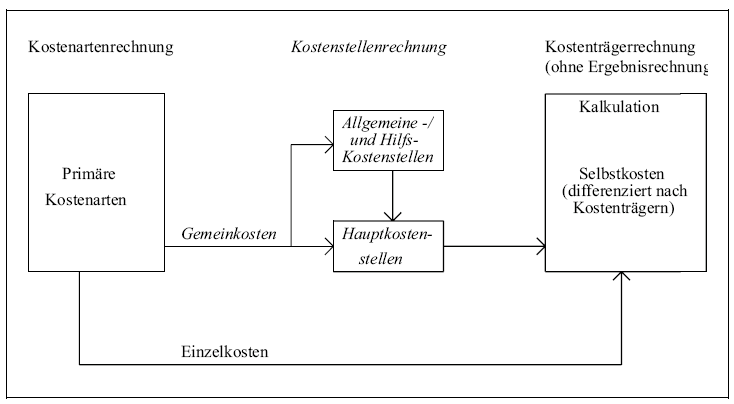
\includegraphics[scale=0.5]{bilder/kostenstellenrechnung_ueberblick.png}
 \end{center}
\end{figure}
%%%%%%%%%%%%%%%%%%%%%%%%%%%%%%%%%%%%%%%

\subsubsection*{Kostenstellenplan}

Illustration der Gemeinkostenverrechnung
\begin{itemize}
	\item 300.000 Euro Fertigungsmaterial (= Materialeinzelkosten)
	\item 50.000 Euro Fertigungslöhne
	\item 200.000 Euro Gemeinkosten
	\item Produziert werden die beiden Enderzeugnisse A und B
\end{itemize} 

\newpage
Kostenstellenplan:

%%%%%%%%%%%%%%%%%%%%%%%%%%%%%%%%%%%%%%%
%% Bild: Portfolio
\begin{figure}[h]
 \begin{center}
   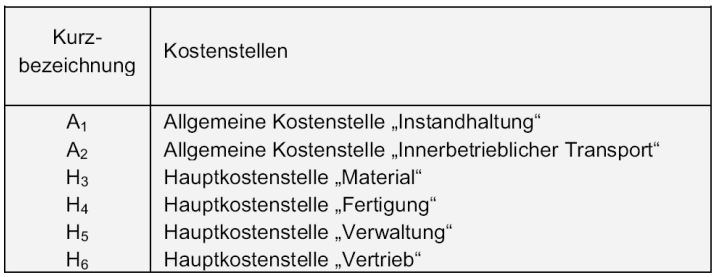
\includegraphics[scale=0.5]{bilder/kostenstellenplan.png}
 \end{center}
\end{figure}
%%%%%%%%%%%%%%%%%%%%%%%%%%%%%%%%%%%%%%%

%%%%%%%%%%%%%%%%%%%%%%%%%%%%%%%%%%%%%%%
%% Bild: Portfolio
\begin{figure}[h]
 \begin{center}
   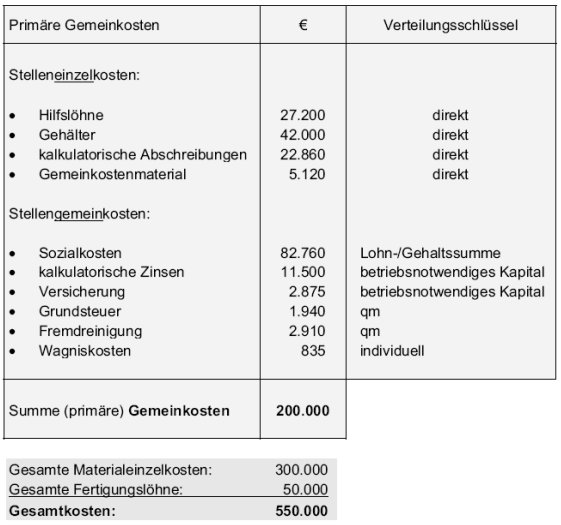
\includegraphics[scale=0.5]{bilder/gemeinkosten.png}
 \end{center}
\end{figure}
%%%%%%%%%%%%%%%%%%%%%%%%%%%%%%%%%%%%%%%

\subsubsection*{Betriebsabrechnungsbogen}

%%%%%%%%%%%%%%%%%%%%%%%%%%%%%%%%%%%%%%%
%% Bild: Portfolio
\begin{figure}[h]
 \begin{center}
   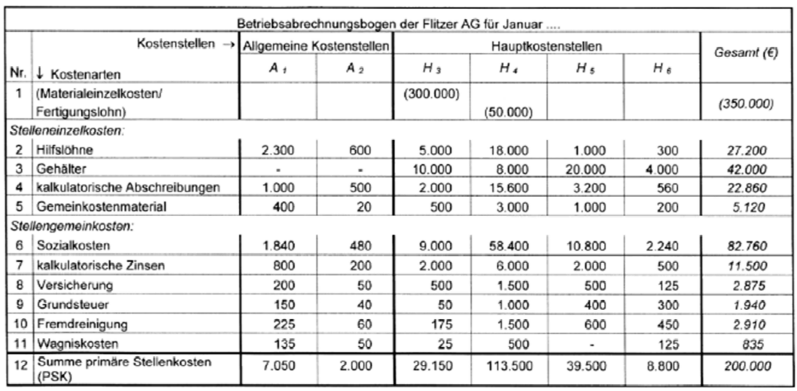
\includegraphics[scale=0.5]{bilder/bab.png}
 \end{center}
\end{figure}
%%%%%%%%%%%%%%%%%%%%%%%%%%%%%%%%%%%%%%%
\newpage 

\subsubsection*{Innerbetriebliche Leistungsverrechnung}
Nach Verteilung der Gemeinkosten sind Kosten angefallen auf:
\begin{itemize}
	\item Allgemeine Kostenstellen (indirekte Leistungen)
	\item Hauptkostenstellen (direkte Leistungen)
\end{itemize}

Die indirekte Leistungen missen nun auf Kostenstellen verrechnet werden für die sie erbracht wurden\\
$\rightarrow$ Abgebende Kostenstelle wird entlastet, empfangende Kostenstelle belastet

Nach Verrechnung keine Gemeinkosten mehr auf Allgemeine-/Hilfskostenstellen\\
$\rightarrow$ gesamte Kosten verteilen sich auf Hauptkostenstelle

Leistungsaustauschmatrix - Berechnung:

%%%%%%%%%%%%%%%%%%%%%%%%%%%%%%%%%%%%%%%
%% Bild: Portfolio
\begin{figure}[h]
 \begin{center}
   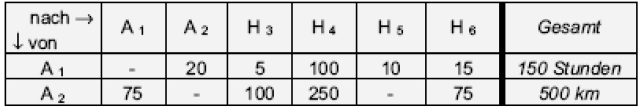
\includegraphics[scale=0.5]{bilder/leistungsaustauschmatrix.png}
 \end{center}
\end{figure}
%%%%%%%%%%%%%%%%%%%%%%%%%%%%%%%%%%%%%%%

%%%%%%%%%%%%%%%%%%%%%%%%%%%%%%%%%%%%%%%
%% Bild: Portfolio
\begin{figure}[h]
 \begin{center}
   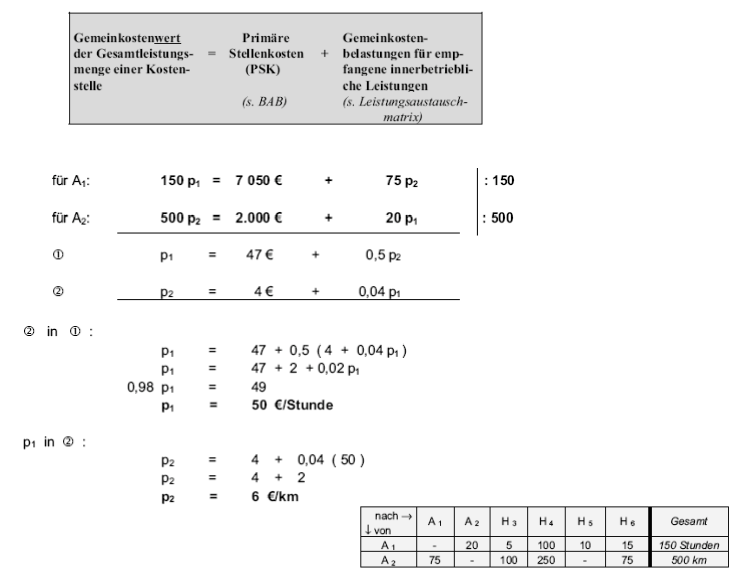
\includegraphics[scale=0.6]{bilder/leistungsverechnung1.png}
 \end{center}
\end{figure}
%%%%%%%%%%%%%%%%%%%%%%%%%%%%%%%%%%%%%%%

%%%%%%%%%%%%%%%%%%%%%%%%%%%%%%%%%%%%%%%
%% Bild: Portfolio
\begin{figure}[h]
 \begin{center}
   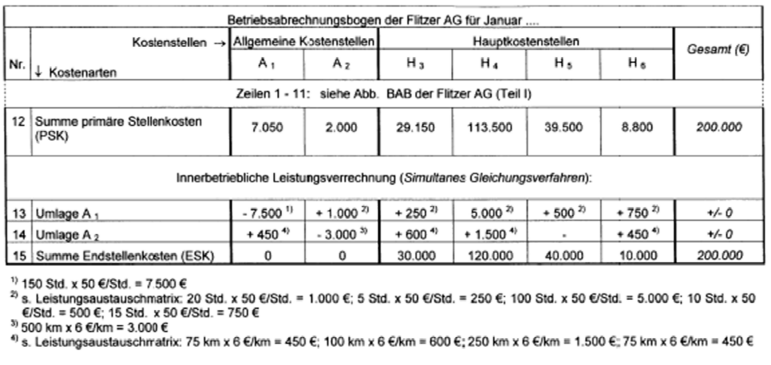
\includegraphics[scale=0.5]{bilder/leistungsverechnung2.png}
 \end{center}
\end{figure}
%%%%%%%%%%%%%%%%%%%%%%%%%%%%%%%%%%%%%%%
\newpage 

\textbf{Ermittlung der Zuschlagssätze} $\rightarrow$ \textbf{Problem}\\
\textit{Auf der Hauptkostenstelle H4 (Fertigung) sind insgesamt 120.000 Euro Kosten angefallen. Da zwei Produkte produziert werden, stellt sich bei der Kalkulation die Frage, wie diese Gemeinkosten auf die beiden Produkte aufzuteilen sind.}

Für die Verteilung wird gesucht:
\begin{itemize}
	\item Eine gemeinsame Verteilungsbasis (Bezugsgröße: Mengen-/Wert- oder Zeitgröße)
	\item Zuschlagsbasis, in direkter Abhängigkeit zu verteilenden Gemeinkosten
\end{itemize}  

Berechnungen

\begin{equation}
\text{Zuschlagssatz} = \frac{\text{Endstellenkosten (ESK) der Hauptkostenstelle}}{\text{Bezugsgröße der Hauptkostenstelle}} \cdot 100
\end{equation}

\begin{equation}
\text{Zuschlagssatz} = \frac{\text{Endstellenkosten (ESK) der Hauptkostenstelle}}{\text{Bezugsgröße der Hauptkostenstelle}} \cdot 100
\end{equation}

\begin{equation}
\text{Zuschlagssatz} = \frac{\text{Endstellenkosten (ESK) der Hauptkostenstelle}}{\text{Bezugsgröße der Hauptkostenstelle}} \cdot 100
\end{equation}

\begin{equation}
\text{Materialgemeinkostenzuschlagssatz} = \frac{\text{Materialgemeinkosten}}{\text{Materialeinzelkosten}} \cdot 100
\end{equation}

\begin{equation}
\text{Fertigungsgemeinkostenzuschlagssatz} = \frac{\text{Fertigungsgemeinkosten}}{\text{Fertigungseinzelkosten}} \cdot 100
\end{equation}

\begin{equation}
\text{Verwaltungskostenzuschlagssatz} = \frac{\text{Verwaltungskosten}}{\text{Herstellkosten}} \cdot 100
\end{equation}

\begin{equation}
\text{Vertriebsgemeinkostenzuschlagssatz} = \frac{\text{Vertriebsgemeinkosten}}{\text{Herstellkosten}} \cdot 100
\end{equation}

\begin{equation}
\text{Forschungs- und Entwicklungsgemeinkostenzuschlagssatz} = \frac{\text{FuE-Gemeinkosten}}{\text{Herstellkosten}} \cdot 100
\end{equation}

%%%%%%%%%%%%%%%%%%%%%%%%%%%%%%%%%%%%%%%
%% Bild: Portfolio
\begin{figure}[h]
 \begin{center}
   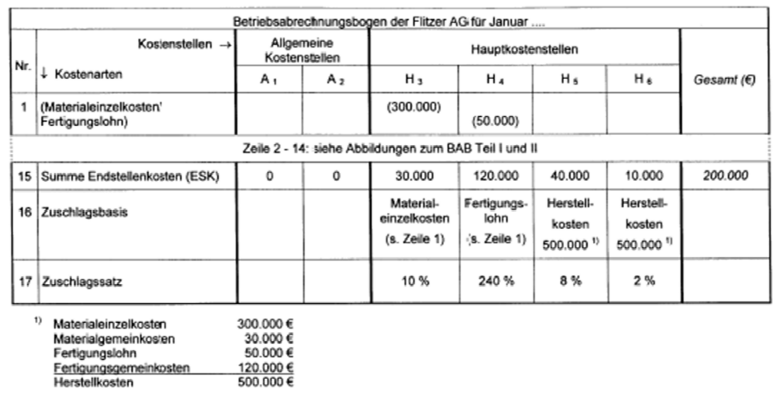
\includegraphics[scale=0.5]{bilder/zuschlagssaetze.png}
 \end{center}
\end{figure}
%%%%%%%%%%%%%%%%%%%%%%%%%%%%%%%%%%%%%%%

\newpage
\subsection{Kostenträgerrechnung (Vollkostenkalkulation)}

\subsubsection*{Grundschema der Zuschlagskalkulation}

%%%%%%%%%%%%%%%%%%%%%%%%%%%%%%%%%%%%%%%
%% Bild: Portfolio
\begin{figure}[h]
 \begin{center}
   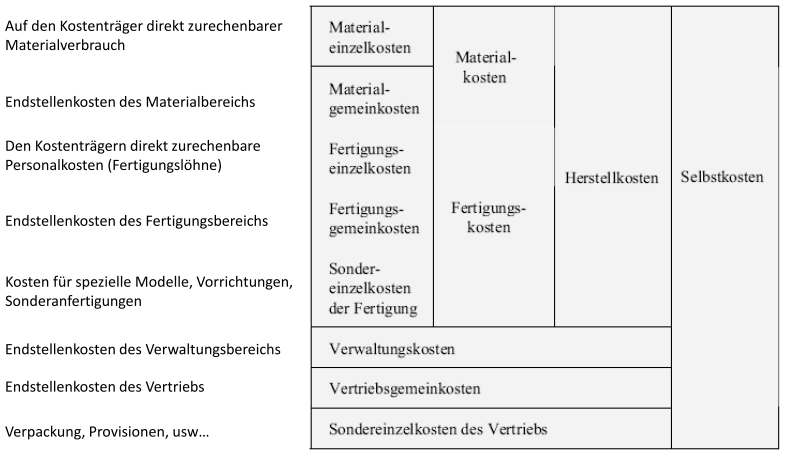
\includegraphics[scale=0.5]{bilder/grundschema_zuschlagskalkulation.png}
 \end{center}
\end{figure}
%%%%%%%%%%%%%%%%%%%%%%%%%%%%%%%%%%%%%%%

\underline{Beispiel der Zuschlagskalkulation:}

%%%%%%%%%%%%%%%%%%%%%%%%%%%%%%%%%%%%%%%
%% Bild: Portfolio
\begin{figure}[h]
 \begin{center}
   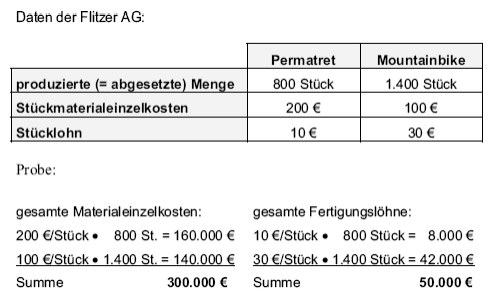
\includegraphics[scale=0.6]{bilder/beispiel_zuschlagskalkulation.png}
 \end{center}
\end{figure}
%%%%%%%%%%%%%%%%%%%%%%%%%%%%%%%%%%%%%%%

%%%%%%%%%%%%%%%%%%%%%%%%%%%%%%%%%%%%%%%
%% Bild: Portfolio
\begin{figure}[h]
 \begin{center}
   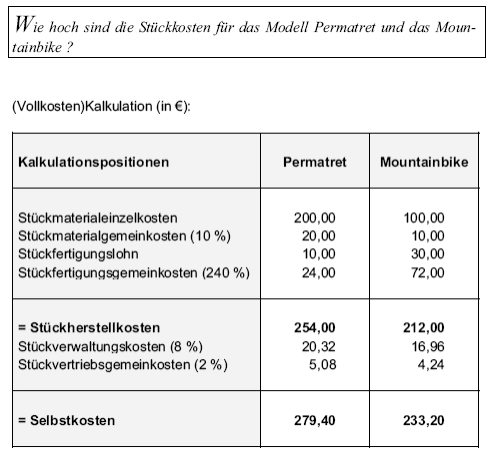
\includegraphics[scale=0.5]{bilder/beispiel_zuschlagskalkulation2.png}
 \end{center}
\end{figure}
%%%%%%%%%%%%%%%%%%%%%%%%%%%%%%%%%%%%%%%

\subsubsection*{Kurzfristige Erfolgsrechnung - Betriebsergebnisrechnung}

\textbf{Gesamtkostenverfahren}\\
Zur Ermittlung des betrieblichen Erfolgs ist es erforderlich, den herstellungs- und absatzbedingten Kosten die entsprechenden Erlöse gegenüber zu stellen

$\rightarrow$ monatliche Ermittlung des Erfolgs = kurzfristige Erfolgsrechnung\\
$\rightarrow$ Gesamtkostenverfahren: Gegenüberstellung gesamte Erlöse/gesamten Kosten in Abrechnungsperiode

\begin{equation}
\begin{aligned}
 & \text{(Umsatz-) Erlöse der Periode}\\
 + & \text{Bestandserhöhung an fertigen und unfertigen Leistungen (bewertet zu Herstellungskosten)}\\
 - & \text{Bestandsminderungen an fertigen und unfertigen Leistungen (bewertet zu Herstellungskosten)}\\
 - & \text{Gesamtkosten der Periode gegliedert nach Kostenarten}\\\hline
 = & \text{Betriebsergebnis}
 & \end{aligned}
\end{equation}

\textbf{Umsatzkostenverfahren}\\
Die gesamten Umsatzerlöse (pro Erzeugnis) werden die gesamten Selbstkosten (pro Erzeugnis) gegenübergestellt. Die Selbstkosten beziehen sich auf die abgesetzte Menge (Umsatz) daher Umsatzkostenverfahren.

\begin{equation}
\begin{aligned}
 & \text{Umsatzerlöse der in der Periode abgesetzten Erzeugnisse, gegliedert nach Erzeugnisarten}\\
 - & \text{Selbstkosten der in der periode abgesetzten Erzeugnisse (=Umsatzkosten), gegliedert nach Erzeugnisarten}\\\hline
 = & \text{Betriebsergebnis}
 & \end{aligned}
\end{equation}

$\rightarrow$ stellt Kosten- und Erlösseite getrennt nach Erzeugnissen auf\\
$\rightarrow$ Zusammensetzung des Gesamterfolgs wird sichtbar

\underline{Beispiel:}

%%%%%%%%%%%%%%%%%%%%%%%%%%%%%%%%%%%%%%%
%% Bild: Portfolio
\begin{figure}[h]
 \begin{center}
   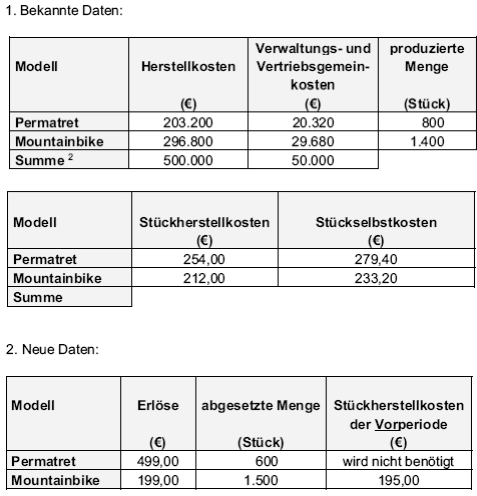
\includegraphics[scale=0.5]{bilder/beispiel_betriebsergebnisrechnung1.png}
 \end{center}
\end{figure}
%%%%%%%%%%%%%%%%%%%%%%%%%%%%%%%%%%%%%%%

%%%%%%%%%%%%%%%%%%%%%%%%%%%%%%%%%%%%%%%
%% Bild: Portfolio
\begin{figure}[h]
 \begin{center}
   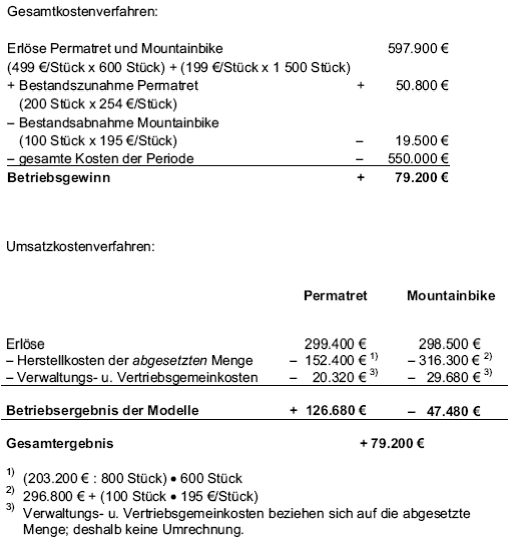
\includegraphics[scale=0.5]{bilder/beispiel_betriebsergebnisrechnung2.png}
 \end{center}
\end{figure}
%%%%%%%%%%%%%%%%%%%%%%%%%%%%%%%%%%%%%%%

\subsubsection*{Kostenkontrolle}
Normalkosten stellen Bezugspunkt zur Kostenkontrolle dar
\begin{itemize}
	\item Normalkosten: Durchschnittliche Ist-Kosten bezogen auf die aktuelle Beschäftigung
	\item Vergleich der Ist-Kosten mit den Normalkosten ergibt Über- oder Unterdeckung
	\item Normalkosten sind leicht zu ermitteln, beinhalten aber Unwirtschaftlichkeiten, da es sich um Ist-Kosten handelt
\end{itemize}
$\rightarrow$ wirksamere Kostenkontrolle durch eine Kostenplanung (Plankosten = erwartete und bei normalem, ordnungsgemäßen Verlauf entstehende Kosten)\\
$\rightarrow$ Berücksichtigung der Ist-Beschäftigung (Plankosten basieren auf einer Planbeschäftigung und sind daher umzurechnen (= Sollkosten)

\begin{equation}
 \text{Sollkosten} =  \text{Plankosten} + \frac{\text{variable Plankosten} \cdot \text{Ist-Beschäftigung}}{\text{Planbeschäftigung}} 
\end{equation}

\textbf{Weitere Berechnungen}

\begin{equation}
 \text{Planverrechnungssatz} = \frac{\text{Plankosten}}{\text{Planbeschäftigung}} 
\end{equation}

\begin{equation}
 \text{Verrechnete Plankosten} = \text{Planverrechnungssatz} \cdot \text{Ist-Beschäftigung} 
\end{equation}

\textbf{Berechnung der Abweichungen}

\begin{equation}
 \text{Verbrauchsabweichung} = \text{Ist-Kosten} - \text{Soll-Kosten} 
\end{equation}

\begin{equation}
 \text{Beschäftigungsabweichung} = \text{Soll-Kosten} - \text{Verrechnete-Plankosten} 
\end{equation}

\underline{Beispiel:}

Ausgangsdaten
\begin{itemize}
	\item Planbeschäftigung: 2.000 Stück
	\item Plankosten: 120.000 Euro (davon 30.000 Euro Fixkosten)
	\item Ist-Beschäftigung: 2.200 Stück
	\item Ist-Kosten: 139.000 Euro
\end{itemize}

Berechnung der der Sollkosten (Plankosten auf Basis der Ist-Beschäftigung)
\[
\text{Soll-Kosten} = 30.000 + \frac{(90.000 \cdot 2.200)}{2.000} = 129.000 \quad \text{Euro}
\]

Verbrauchsabweichung
\[
\begin{aligned}
 & \text{Ist-Kosten} = \text{Ist-Menge} \cdot \text{Planwert}\\
 - & \text{Soll-Kosten} = \text{Soll-Menge} \cdot \text{Planwert}\\\hline
 = & \text{Verbrauchsabweichung}
 & \end{aligned}
\]

\[
\text{Verbrauchsabweichung} = 139.000 - 129.000 = 10.000 \quad \text{Euro}
\]

Beschäftigungsabweichung

\[
\text{Planverrechnungssatz} = \frac{120.000\quad \text{Euro}}{2000\quad \text{Stück}} = 60\quad \text{Euro/Stück}
\]

\[
\text{Tatsächlich produziert} = 2.200\quad \text{Stück} \cdot 60\quad \text{Euro/Stück} = 132.000\quad \text{Euro}
\]

\[
\text{Beschäftigungsabweichung} = 129.000\quad \text{Euro} - 132.000\quad \text{Euro} = -3.000\quad \text{Euro}
\]
Die Beschäftigungsabweichung sagt aus, wie viele Fixkosten bei Überbeschäftigung zu viel verrechnet werden

\[
\text{Gesamtabweichung} = 10.000\quad \text{Euro} + (-3.000\quad \text{Euro}) = 7.000\quad \text{Euro}
\]

\subsection{Teilkostenrechnung/Deckungsbeitragsrechnung}

Die Vollkostenrechnung verrechnet alle Kosten auf die Produkte\\
$\rightarrow$ langfristige Preisuntergrenze\\
Probleme: Fixe Gemeinkostenbestandteile werden wie variable Kosten behandelt

In Teilkostenrechnung werden fixe Kosten nicht mehr in Erzeugnisse kalkuliert, sondern als Periodenkosten in das Betriebsergebnis eingestellt

%%%%%%%%%%%%%%%%%%%%%%%%%%%%%%%%%%%%%%%
%% Bild: Portfolio
\begin{figure}[h]
 \begin{center}
   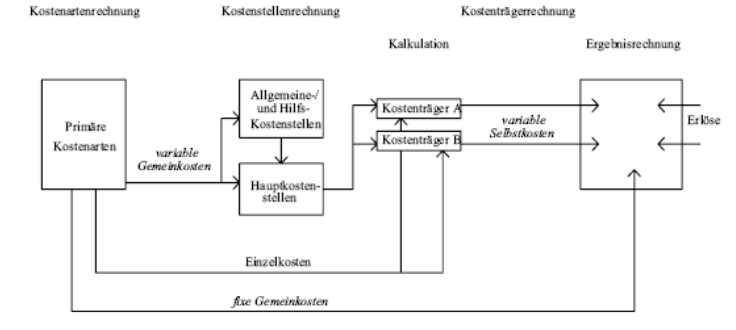
\includegraphics[scale=0.5]{bilder/teilkostenrechnung.png}
 \end{center}
\end{figure}
%%%%%%%%%%%%%%%%%%%%%%%%%%%%%%%%%%%%%%%

%%%%%%%%%%%%%%%%%%%%%%%%%%%%%%%%%%%%%%%
%% Bild: Portfolio
\begin{figure}[h]
 \begin{center}
   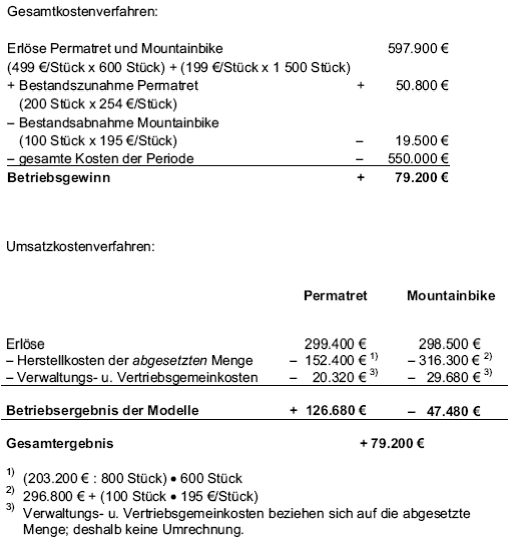
\includegraphics[scale=0.5]{bilder/beispiel_betriebsergebnisrechnung2.png}
 \end{center}
\end{figure}
%%%%%%%%%%%%%%%%%%%%%%%%%%%%%%%%%%%%%%%

%%%%%%%%%%%%%%%%%%%%%%%%%%%%%%%%%%%%%%%
%% Bild: Portfolio
\begin{figure}[h]
 \begin{center}
   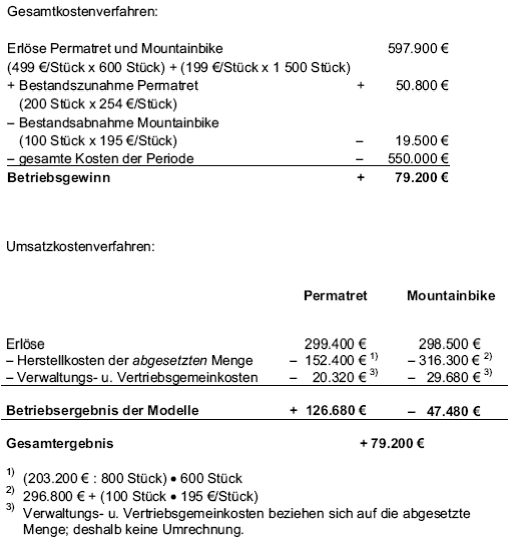
\includegraphics[scale=0.5]{bilder/beispiel_betriebsergebnisrechnung2.png}
 \end{center}
\end{figure}
%%%%%%%%%%%%%%%%%%%%%%%%%%%%%%%%%%%%%%%

%%%%%%%%%%%%%%%%%%%%%%%%%%%%%%%%%%%%%%%
%% Bild: Portfolio
\begin{figure}[h]
 \begin{center}
   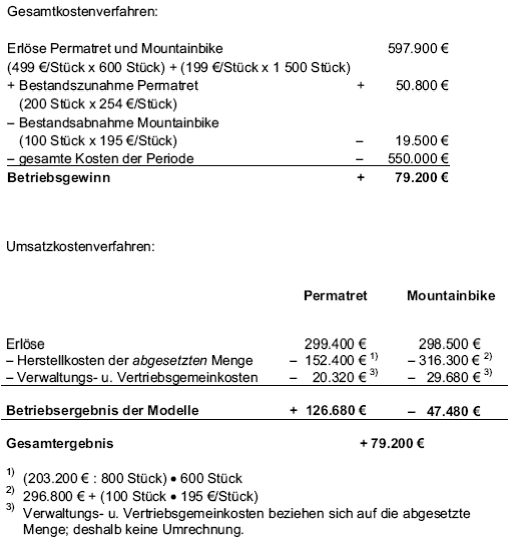
\includegraphics[scale=0.5]{bilder/beispiel_betriebsergebnisrechnung2.png}
 \end{center}
\end{figure}
%%%%%%%%%%%%%%%%%%%%%%%%%%%%%%%%%%%%%%%
\end{document} 

